\graphicspath{{chapters/regularisation}}


\chapter{Regularisation of CCA Models}\label{chap:als}
%\epigraph{All models are wrong, some are useful.}{\textit{G. Box}}
\minitoc
% chktex-file 44 
% chktex-file 3
\section*{Preface}

In this chapter, I build upon my earlier work presented at the OHBM conference and the insights gained from a tutorial paper I co-authored, which included a series of simulations \citep{mihalik2022canonical}.

\section{Introduction}\label{sec:introduction}

This chapter introduces a novel approach for analyzing large-scale neuroimaging datasets, such as the Human Connectome Project (\acrshort{hcp}) and Alzheimer's Disease Neuroimaging Initiative (\acrshort{adni}), to understand the relationship between brain structure, function, and behavior \citep{SMITH2018263,BZDOK2017549,wang2020finding}. These datasets are characterized by a disproportion between the number of subjects and the volume of features, posing a challenge for Canonical Correlation Analysis (CCA) models due to the risk of overfitting and spurious correlations \citep{citation}. For example, the \acrshort{hcp} dataset used in this chapter contains 1003 subjects and 19,900 features in the functional MRI (fMRI) view alone while the \acrshort{adni} dataset contains 592 subjects and  168,130 features in the structural MRI (sMRI) view alone.

In response to the reproducibility crisis in neuroscience \citep{button2013power}, this chapter focuses on enhancing the generalizability of CCA models through regularization, a technique that introduces a bias towards more interpretable and generalizable models \citep{engl1996regularisation,bzdok2019towards}. Traditional regularization methods in CCA, such as 'sparse CCA' with Partial Least Squares (PLS) objectives, are limited by their inherent bias towards the largest principal components \citep{citation}.

To overcome these limitations, we propose the Flexible Regularised Alternating Least Squares (FRALS) framework for CCA. FRALS allows for the integration of various regularized least squares solvers, particularly emphasizing the elastic net penalty, which combines L2 and L1 penalties. This method controls bias and promotes sparsity in model weights, advancing beyond previous sparse Brain-Behavior analysis methods.

Our application of the FRALS framework with Elastic Net regularization to the \acrshort{hcp} and \acrshort{adni} datasets showcases its effectiveness in enhancing out-of-sample canonical correlation compared to traditional CCA models \citep{citation}. Additionally, FRALS uncovers new modes of variation in brain-behavior relationships.

In essence, this chapter presents FRALS as a robust, innovative solution for the analysis of high-dimensional neuroimaging datasets, significantly improving the reliability and interpretability of Brain-Behavior correlations.

\section{Background: Regularisation for High-Dimensional and Structured Data}\label{sec:background}

In this section, we review a number of regularisation techniques that have been applied to CCA and related methods.

\subsection{The Bias-Variance Tradeoff}

A key principle in machine learning is the bias-variance tradeoff.
This concept posits that a tradeoff exists between the bias and variance of a model: high-bias models typically exhibit low variance, and vice versa.
High-bias models are generally simpler and more stable, but they might oversimplify the problem, leading to underfitting.
Conversely, low-bias, complex models are sensitive to data changes and prone to overfitting.
As the number of features increases, there are more parameters to estimate, and models tend to become more complex, leading to higher variance and lower bias.
This relationship highlights the importance of balancing model complexity to avoid overfitting, particularly in high-dimensional scenarios with a low signal-to-noise ratio \citep{mcintosh2021comparison}\footnote{It's worth noting that the number of model parameters, often used as a proxy for complexity, does not always directly correlate with model behavior, as illustrated by the `double descent' phenomenon.}.
Regularisation can be understood as a method for reducing the variance of a model by introducing a bias towards simpler models.
This means regularisation can improve the generalizability of models in high-dimensional settings.

\paragraph{Implicit and Explicit Regularisation}

We can implement regularisation in two different ways.
\textit{Explicit} regularisation is achieved by adding a penalty term to the objective function. Weights the objective function against a term that penalises complexity.

\textit{Implicit} regularisation is achieved by changing the optimisation algorithm and can include dimensionality and feature engineering techniques.

\subsection{Shrinkage Regularisation}

Shrinkage regularisation is a form of regularisation that penalises the magnitude of the model parameters.
This technique is particularly effective in enhancing the performance of linear models in situations characterised by high dimensionality, multicollinearity, or low signal-to-noise ratios.

In high-dimensional situations where the number of features exceeds the number of observations in either view, Like Linear Regression, Canonical Correlation Analysis is non-identifiable, meaning there is no unique solution.
This is because we can find perfectly correlated latent variables using a linear combination of the features, but there are many different linear combinations that will achieve this.
Some of these linear combinations will generalize better than others, but there is no way to distinguish between them using the training data alone.

Even in low-dimensional situations, if features exhibit multicollinearity, they can also be non-identifiable or, at best, estimates of the parameters are unstable.
Mathematically, this is because in both cases the covariance matrix of the features is not full rank and therefore is not invertible (non-identifiable) or ill-conditioned (matrix inversion is unstable).
To capture this intuition, if two features are perfectly correlated, the model is not identifiable (has no unique solution) because we can arbitrarily swap the \gls{weights} between the two features without changing the latent variables (\acrshort{cca}) or the predictions (regression).
In practice, features are rarely perfectly correlated, but even when features are highly correlated, the model can be unstable \citep{mihalik2020multiple}, and small changes in the data can lead to large changes in the model parameters.
Once again, some of these linear combinations will generalize better than others, but we might expect a model to generalize better if it spreads the \gls{weights} across the correlated features rather than concentrating them on a single feature.

Finally, even in low-dimensional settings with little multicollinearity, the model parameters can be sensitive to noise in the data, and once again small changes in the data can lead to large changes in the model parameters.
For example, parameters associated with noisy features might `cancel out' in the training set, but not in the test set, leading to poor generalisation.

The premise of shrinkage regularisation in all these cases is that the latent variables or predictions are too sensitive to small changes in the data because the model parameters are too large.
Shrinkage regularisation works by shrinking the model parameters towards zero, so that small changes in the data do not lead to large changes in the model estimates.

\paragraph{PLS as Shrinkage Regularisation} PLS can be interpreted as a form of shrinkage regularisation applied to CCA. We can explain this by considering an analogy between CCA and \textit{Linear Regression}\footnote{indeed Linear Regression is a special case of CCA where \(X^{(2)}\) has one feature}.

In Linear Regression, the ridge regression solution is given by:
\begin{align}
    \hat{\beta}_{\text{ridge}} = ((1-c)\Sigma_{X,X} + c I)^{-1} \Sigma_{X,y}
\end{align}
Where \(c\) is the regularisation parameter between 0 and 1\footnote{It is more common to see $(\Sigma_{X,X} + c I)^{-1} \Sigma_{X,y}$ but these are equivalent up to a scalar factor and this form helps us later on}.
The ridge penalty acts in three important ways:
\begin{itemize}
    \item It shrinks the \gls{weights} towards zero.
    \item It shrinks the \gls{weights} of correlated features towards each other.
    \item It biases the solution to high covariance directions rather than high correlation directions.
\end{itemize}

As $c$ becomes large, $\lim_{c \to \infty} (\Sigma_{X,X} + c I)^{-1} = (c I)^{-1}$
, so that $\hat{\beta}_{\text{ridge}}=\frac{\Sigma_{X,y}}{c}$, which is precisely the covariance of the features of $X$ with $Y$ scaled by $c$ (and shrunk towards zero for $c \geq 1$).
Notice that the ridge regression solution is no longer sensitive to the correlation of features in $X$.
Additionally, notice that for sufficiently large $c$, $(\Sigma_{X,X} + c I)$ is invertible even if $\Sigma_{X,X}$ is not invertible, so that ridge regression is always identifiable even when the number of features exceeds the number of observations.

Now consider the CCA problem.
Firstly, recall that PLS and CCA are equivalent up to a scaling when the covariance matrices are identity matrices, a similar relationship to the relationship between Linear and Ridge Regression.
Consider the well-known form of CCA given in equation~\ref{eq:cca}\citep{mihalik2022canonical} (formed by reparameterizing \(u\sps{i}=(\Sigma_{ii})^{-\frac{1}{2}}u\sps{i}\)):

\begin{align}
    \label{eq:cca}
    & u_{\text{opt}}=\underset{u}{\mathrm{argmax}}\{ u\spsT{1}(\Sigma_{11}+ c I)^{-\frac{1}{2}}\Sigma_{12}(\Sigma_{22}+c I)^{-\frac{1}{2}}u\sps{2} \} \\
    & \text{subject to:} \notag \\
    & u\spsT{1}u\sps{1}=1, u\spsT{2}u\sps{2}=1 \notag
\end{align}

As we increase $c$, $\lim_{c \to \infty} (\Sigma_{ii}+ c I)^{-\frac{1}{2}}= (c I)^{-1}$ so that the objective approaches:

\begin{align}
    & u_{\text{opt}}=\underset{u}{\mathrm{argmax}}\{ u\spsT{1}(c I)^{-1}\Sigma_{12}(c I)^{-1}u\sps{2} \} \\
    & \text{subject to:} \notag \\
    & u\spsT{1}u\sps{1}=1, u\spsT{2}u\sps{1}=1 \notag
\end{align}

Which is precisely the PLS objective and constraints with an arbitrary scaling of the covariance matrix $\Sigma_{12}$ by $\frac{1}{c^2}$.
For this reason, we can consider PLS as an explicit shrinkage method for CCA, equivalent to adding a maximal ridge regularisation term.
The downside of using PLS as a regularised CCA is precisely its very high bias.
By strongly guiding the model towards high covariance solutions, it strongly biases the solution towards only the largest principal components.
But what if the correlation between the views is not concentrated in the largest principal components?
Although one would rarely resort to maximally regularised ridge regression except in extremely low sample sizes or high-dimensional data, it has become almost standard practice to use PLS in neuroimaging and genetics \citep{cruciani2022pls, krishnan2011partial}.
One of the core contributions of this chapter will be to demonstrate that PLS is usually a poor choice for regularisation even in these very high-dimensional settings and that more nuanced regularisation methods can offer significant improvements in performance and interpretability.
PLS is evidently not a nuanced tool for regularisation because it offers no control over the degree of regularisation applied.

\paragraph{Ridge Regularisation} For this reason, \citet{vinod1976canonical} proposed the \textit{Canonical Ridge} or \textit{Ridge CCA}, which combined the PLS and CCA constraints in a single constrained optimisation:

\begin{align}
    & u\sps{1}_{\text{opt}} = \underset{u\sps{1}}{\mathrm{argmax}} \{ u\spsT{1} \hat{\Sigma_{12}} u\sps{2} \} \\
    & \text{subject to:} \notag \\
    & (1 - c_1) u\spsT{1} \hat{\Sigma_{11}} u\sps{1} + c_1 u\spsT{1} u\sps{1} = 1 \notag \\
    & (1 - c_2) u\spsT{2} \hat{\Sigma_{22}} u\sps{2} + c_2 u\spsT{2} u\sps{2} = 1 \notag
\end{align}

Where $c_1$ and $\tau_2$ are the ridge regularisation parameters for the first and second views respectively.
By tuning these parameters, we can control the degree of regularisation applied to each view independently.
If we set $c_1$ and $c_2$ to zero, we recover the standard CCA objective while if we set $c_1$ and $c_2$ to one, we recover the PLS objective.
This allows us to interpolate between the two extremes, allowing us to control the level of shrinkage and therefore the level of bias towards the largest principal components. Ridge CCA has been shown to be effective for neuroimaging data for both CCA \citep{tenenhaus2011regularized, tuzhilina2023canonical, hardoon2004canonical} and Kernel CCA \citep{hardoon2007unsupervised}.

\paragraph{PCA-CCA} PCA be can be used as an implicit regularisation method for CCA.

Most obviously, by using only the first \( k \) principal components of each view as the input to CCA, we can reduce the dimensionality of the data and therefore reduce the number of parameters in the model.
Moreover, by working with the principal components, we remove the correlation between the features, which can improve the conditioning of the problem.
While PCA and Independent Component Analysis (ICA) are often used as preprocessing steps for CCA, they can also be used as regularisation methods in their own right.
Of particular note in neuroimaging are studies with a data-driven approach to the PCA step, where the number of principal components is chosen based on the data \citep{liu2022improved, mihalik_canonical_2022}.

\paragraph{}

\paragraph{A Visual Comparison of Shrinkage Techniques}

The distinct effects of Ridge and PCA on the eigenvalues of the effective covariance matrices can be clearly visualised with a simple visualisation.
We plot the eigenvalues of covariance matrices as perceived by models with different regularisation techniques \footnote{e.g. the eigenvalues of $(1 - c_i) \hat{\Sigma_{ii}} + c_i I$ for ridge and $\hat{\Sigma_{ii}}$ truncated to include only the largest $k$ principal components for PCA}.
As shown in Figure~\ref{fig:shrinkage}, Ridge regularisation reduces the magnitude of the largest eigenvalues in the effective covariance matrix towards 1, and increases the magnitude of the smallest eigenvalues towards 1.
On the other hand, PCA-CCA, leaves the largest eigenvalues unchanged, and ignores the smallest eigenvalues (we could have represented this by setting them to infinity).

\begin{figure}[h]
    \centering
    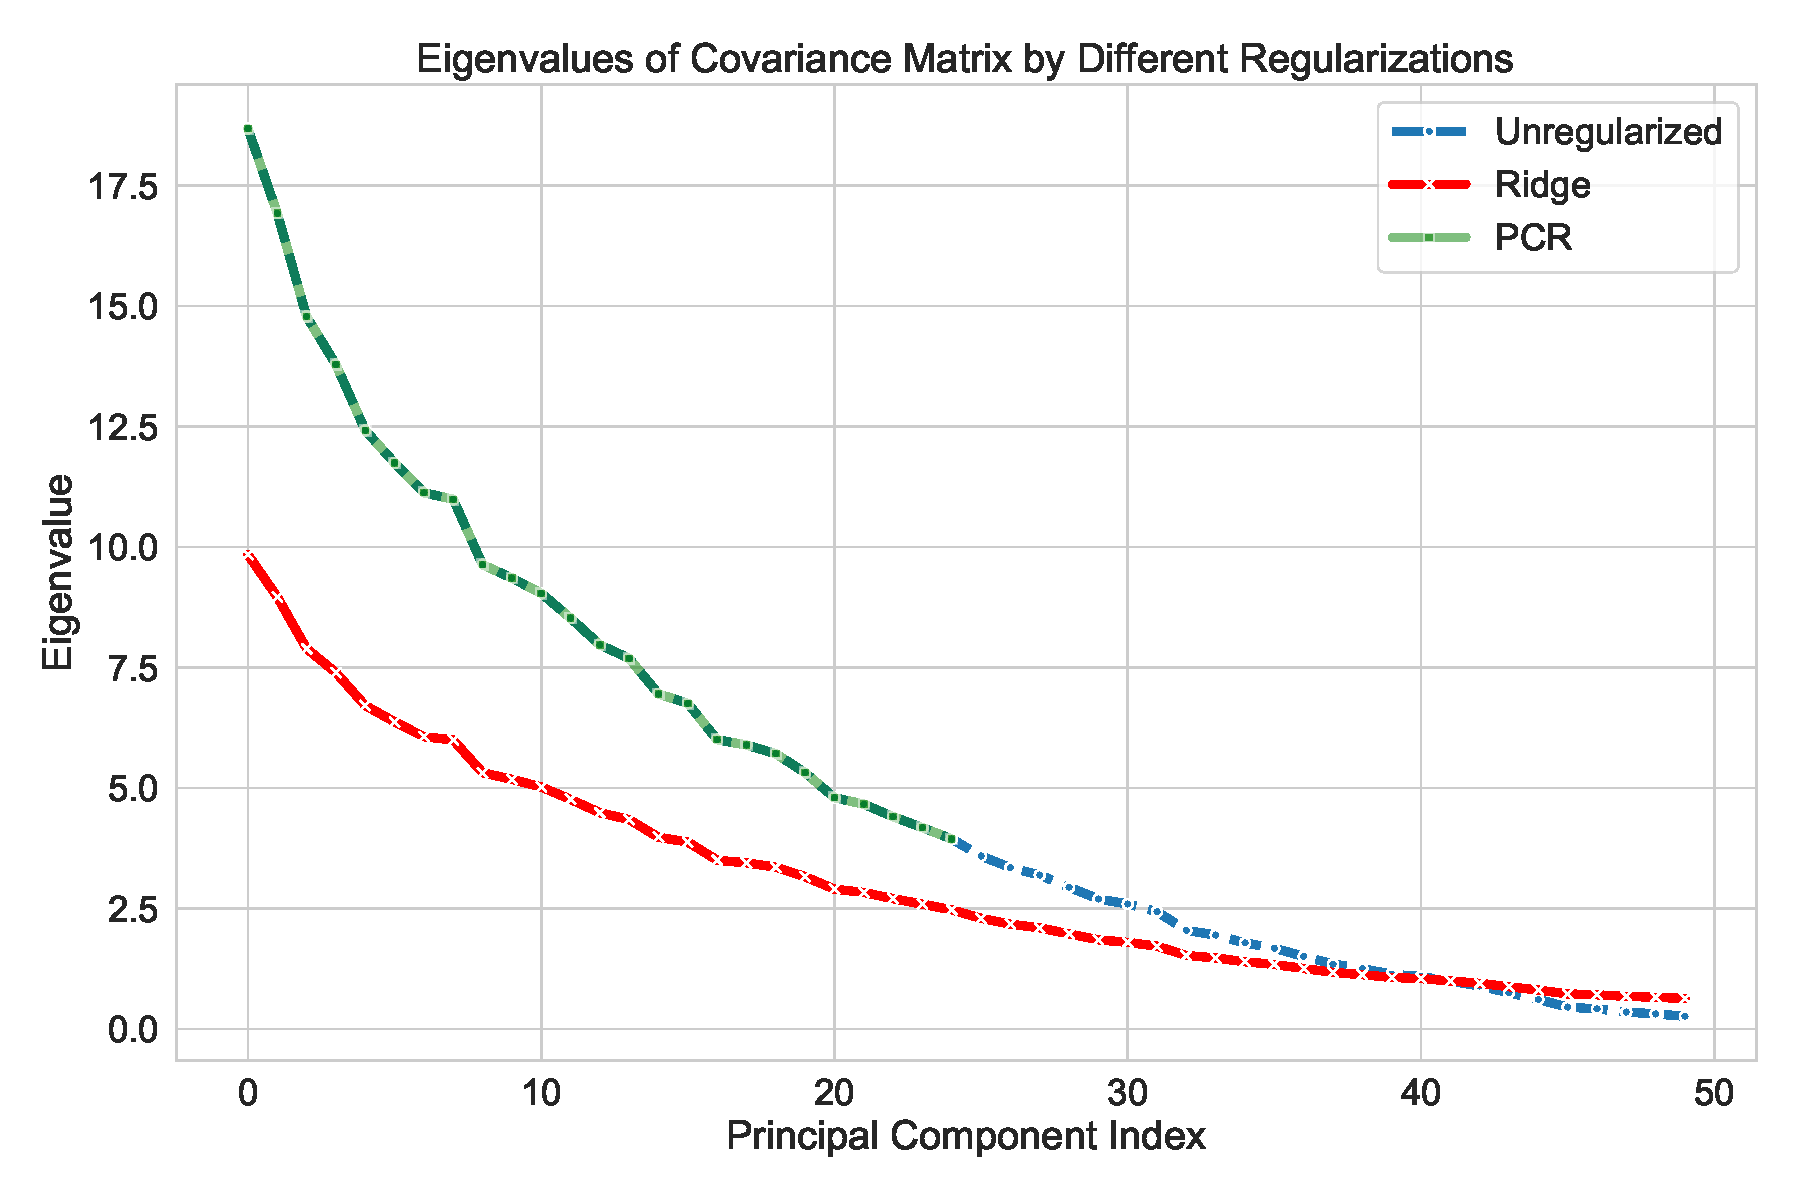
\includegraphics[width=0.8\textwidth]{figures/shrinkage/shrinkage}
    \caption{Comparison of the effect of OLS, Ridge, and PCA regularisation on the eigenvalues of the covariance matrix.}\label{fig:shrinkage}
\end{figure}

When these effective covariance matrices are inverted to form the CCA objective, these effects are reversed.
Ridge regularisation increases the magnitude of the weights associated with the largest eigenvalues and decreases the magnitude of the smallest eigenvalues.
PCA maintains the weights associated with the largest eigenvalues and sets the weights associated with the smallest eigenvalues to zero.
The visualisation underscores the intrinsic nature of each regularisation method:
\begin{itemize}
    \item \textbf{Unregularised}: Presents the unaltered spectrum, making it susceptible to noise but preserving potential subtle patterns.
    \item \textbf{Ridge}: Warps the spectrum, shrinking the largest eigenvalues and expanding the smallest eigenvalues, potentially missing subtle patterns but offering a cleaner representation of stronger associations.
    \item \textbf{PCA}: Truncates the spectrum, ignoring the smallest eigenvalues and preserving the largest eigenvalues, potentially missing subtle patterns but offering a cleaner representation of stronger associations.
\end{itemize}

However, while these shrinkage techniques can improve the performance of CCA, they do not obviously improve the interpretability of the results.
Weights are shrunk towards zero, but they are not set to zero.
This means that the model still uses all the features, and the results are not sparse.

\subsection{Sparse Regularisation}

Sparse regularisation is a powerful tool for improving the performance and interpretability of linear models.
Sparse regularisation encourages the model to use only a subset of the features, which can both help to avoid overfitting and improve the interpretability of the model.
Sparse regularisation works on the premise that only a subset of the features are relevant to the model.
Sparsity is typically achieved by adding either an L1 penalty or constraint\footnote{The L0 norm of the weight vector is the number of non-zero elements in the vector and is arguably a closer match to the goal, but the L0 norm is (a) not a proper norm in the mathematical sense and (b) not convex and so is difficult to optimize.}.
The L1 penalty is defined as:

\begin{align}
    \|u\|_1 = \sum_i |u_i|
\end{align}

Intuitively, this is the sum of the absolute values of the elements of the vector.
Now, with a foundational understanding of sparse regularisation, we review a number of approaches to adding sparsity to the CCA problem.

\paragraph{Sparse PLS: Penalized Matrix Decomposition}
Penalized Matrix Decomposition (PMD)~\citep{witten2009penalized} provides an approximate solution to the sparse CCA problem by altering the constraints of the classical CCA formulation.
Specifically, PMD replaces the constraints \(u\spsT{i} \hat{\Sigma_{ii}} u\sps{i} = 1\) with the PLS constraints \(u\spsT{i} u\sps{i}= 1\) and additionally imposes \(\|u\spsT{i}\|_1 \leq \tau\).
The optimisation problem for PMD is then given by:

\begin{align}
    & u^{opt}=\underset{u}{\mathrm{argmax}}\{ u\spsT{1} \hat{\Sigma_{12}} u\sps{2} \} \\
    & \text{subject to:} \notag \\
    & u\spsT{1} u\sps{1} = 1 , u\spsT{2} u\sps{2} = 1 \notag \\
    & \|u\sps{1}\|_1 \leq \tau_1 , \|u\sps{2}\|_1 \leq \tau_2 \notag
\end{align}

This Sparse PLS (SPLS) approximation has been highly influential as a form of Sparse CCA because it is extremely computationally efficient method \footnote{it can be solved by a variant of the power method; iteratively multiplying $u\sps{1}$ by $\hat{\Sigma_{12}}$ and soft-thresholding}.
Like the relationship between PLS and CCA, PMD and a form of CCA with constrained L1 norm are equivalent only when the covariance matrices are identity matrices.
There are a number of other sparse CCA methods that employ the PLS approximation \citep{parkhomenko2009sparse, waaijenborg2008quantifying, lindenbaum2021l0}.
However, while the PLS approximation is efficient, it means these methods inherit a bias towards the largest principal components from PLS.

To address these problems and truly tackle the sparse CCA optimisation, another class of approaches have adopted a penalised least squares approach.

\paragraph{Sparse CCA: Least Squares Approaches}

It is well known that the CCA problem can be formulated as a constrained least squares problem with the intuition that
for \(X\sps{1} u\sps{1}=1\) and \(X\sps{2} u\sps{2}=1\), correlation is maximised when the squared distance
between \(X\sps{1} u\sps{1}\) and \(X\sps{2} u\sps{2}\) is minimised. \citep{golub1995canonical} proved the
convergence of a simple algorithm which alternates between solving the least squares problem for \(u\sps{1}\) and
\(u\sps{2}\) while keeping the other fixed.

With this intuition, \cite{wilms2015sparse} and \cite{mai2019iterative} separately proposed iterative penalised least
squares methods for sparse CCA\@.

\begin{align}
    \label{eq:mai}
    u^{opt} &= \underset{u}{\mathrm{argmin}} \left\{ \|X\sps{1}u\sps{1} - X\sps{2}u\sps{2}\|_2^2 + P(u) \right\} \\
    &\text{subject to:} \notag \\
    &u\spsT{1} \hat{\Sigma_{11}} u\sps{1}=1 \notag \\
    &u\spsT{2} \hat{\Sigma_{22}} u\sps{2}=1 \notag
\end{align}

Where \(P(u)\) is a penalty function.
The penalty term can be any function that penalises the norm of the vector \(u\).
\citep{mai2019iterative} proved that solving the subproblems where one of $u\sps{i}$ is fixed is easy for one-homogenous $P$ where
\( P((\mu + 1)\theta) = (\mu + 1)P(\theta) \) which notably includes the lasso penalty.
This means a sparse CCA based
on alternating lasso regressions can be solved relatively efficiently using existing solvers.
However, the one homogenous penalty in practice limits the flexibility of the method.
For example, the elastic net penalty is not one-homogenous and therefore cannot be used with this method.
\citet{6556581} and \cite{Mullins2021} added ridge penalties to the subproblems to improve the conditioning of the problem in a way that could be considered a form of elastic net regularisation but the subproblems no longer correctly optimize the global objective\footnote{when rescaling the penalised solutions back to unit variance}.

\paragraph{Sparse CCA: Proximal Gradient Descent and ADMM}
\citet{kanatsoulis2018structured} proposed solving equation~\ref{eq:mai} for more general classes of $P$ using the alternating direction method of multipliers (ADMM)~\citep{boyd2011distributed}.
\cite{fu2017scalable} propose a regularised CCA based on an alternative classical CCA formulation, sometimes called the MAXVAR formulation, which views the problem as a constrained least squares with an auxiliary representation $T$\citep{carroll1968generalisation,kettenring1971canonical}.

\begin{align}
    \label{eq:fu}
    \underset{U, T}{\mathrm{argmin}}\left\{\sum_i \|X\sps{i} U\sps{i} - T\|_F^2\right\}\\
    \text{subject to: }T^\top T = I\\
\end{align}

In this formulation, \(U\sps{i}\) represents the \gls{weights} for the $i^{\text{th}}$ view, and \(T\) denotes the latent variable matrix.
The premise is that when \(T\) closely mirrors \(X\sps{i} U\sps{i}\) across all \(i\), the scores correlate.
Notably, this method is adaptable to multiple views.
The authors employed proximal gradient descent for regularisation, specifically suited for penalties like the lasso.
While these methods are flexible, they don't have the plug-and-play nature of the penalised least squares methods.
Not just a matter of convenience, this means that these methods are not compatible with existing solvers for regularised least squares problems like for example total variation regularisation solvers in nilearn, which are often highly optimised for specific problems and modalities.

\paragraph{Structured Regularisation}

As highly structured data, linear models using both structural \acrshort{mri} and f\acrshort{mri} data have been shown to benefit from structured regularisation methods but notably these methods have not been applied to CCA.
Total variation regularisation, which biases spatially neighboring weights to be similar, has been shown to improve the performance of PCA \citep{de2017structured} and regression \citep{michel2011total,dohmatob2014benchmarking, baldassarre2012structured}.
Similarly, Laplacian (or \textit{GraphNet}) regularisation, which induces a similar spatial bias with additional smoothness, has been shown to improve the performance of CCA on functional MRI data \citep{grosenick2013interpretable}.

Having discussed the benefits of both shrinkage (e.g., PCA-CCA, Ridge CCA, PLS), sparsity (SPLS, Sparse CCA), and structure (Total Variation, Laplacian) in handling high-dimensional, noisy, and structured data, a natural progression is to integrate these advantages.
Specifically, the challenge lies in creating a framework that allows for users to match the regularisation method to their data and research question, enhancing the interpretability and performance of Brain-Behaviour association models.
The solution?
A method that employs readily available regularised regression solvers, allowing for flexible and tunable regularisation in CCA.
This leads us to propose the Flexible Regularised Alternating Least Squares (FRALS).

\section{Methods - Flexible Regularised Alternating Least Squares (FRALS)}\label{subsec:flexible-regularised-alternating-least-squares-(frals)}

The primary goal of our Flexible Regularised Alternating Least Squares framework is to provide a versatile and user-friendly interface for Canonical Correlation Analysis (CCA). This is achieved by designing the framework to be compatible with any scikit-learn compatible regularised least squares solver. This compatibility is pivotal as it allows researchers and practitioners to leverage the extensive range of solvers available in scikit-learn, a popular machine learning library in Python.

This approach marks a significant departure from traditional methodologies in CCA, which often focused on developing or utilizing specific solvers tailored for particular types of data or computational constraints.
By contrast, \acrshort{frals} democratises access to advanced CCA techniques, allowing users to select solvers that best fit their specific data characteristics, computational needs, or familiarity.
Such flexibility is particularly advantageous in interdisciplinary fields like neuroimaging, where diverse datasets and varying levels of technical expertise are common.

For example, users dealing with high-dimensional, sparse neuroimaging data could opt for solvers optimised for such datasets, while those needing parallel computation for large data sets might choose solvers with GPU acceleration capabilities.
In principle, \acrshort{frals} can even be used with Neural Network-based solvers, which are becoming increasingly popular in machine learning\footnote{Though for reasons that will later become clear, we do not reccommend this!}.
This adaptability enhances \acrshort{frals}' accessibility and future-proofs the framework against evolving computational technologies and data analysis needs.

In the \acrshort{frals} framework, we consider the formulation for a single latent variable \(t\) with regularisation \(\lambda_i P_i\) on the weights \(u^{(i)}\):

\begin{align}
    \underset{u}{\mathrm{argmin}}\left\{\sum_i \|X^{(i)} u^{(i)} - t\|_2^2 + \textcolor{red}{\lambda_i P_i(u^{(i)})} \right\}\\
    \text{subject to: }t^\top t = 1 \notag
\end{align}

This problem can be decomposed into three subproblems.
The first subproblem for the auxiliary variable \(t\):

\begin{align}
    \underset{t}{\mathrm{argmin}}\left\{\sum_i \|X^{(i)} u^{(i)} - t\|_2^2\right\}\\
    \text{subject to: }t^\top t = 1 \notag
\end{align}

is a standard least squares problem and can be solved in closed form by averaging \(X^{(i)} u^{(i)}\) and normalizing i.e. \(t = \frac{\sum_i X^{(i)} u^{(i)}}{\|\sum_i X^{(i)} u^{(i)}\|_2}\).
As shown earlier this makes \(t\) an estimate of the latent variables of a generative CCA model.

The subproblems for the weights \(u^{(i)}\):

\begin{align}
    \underset{u^{(i)}}{\mathrm{argmin}}\left\{\|X^{(i)} u^{(i)} - t\|_2^2 + \textcolor{red}{\lambda_i P_i(u^{(i)})} \right\}
\end{align}

are regularised least squares problems that can be solved using any suitable regularised least squares solver\footnote{We could also in principle replace $X^{(i)} u^{(i)}$ with $f(X^{(i)})$ for any function $f$ including kernels, neural networks, or random forests}.

In this chapter, we illustrate the power of the \acrshort{frals} framework by implementing the well-tested Elastic Net solver from the \texttt{scikit-learn} package~\citep{pedregosa2011scikit}, where \(P_i = \alpha_i \times \text{l1\_ratio} \|u^{(i)}\|_1 + \alpha_i \times (1-\text{l1\_ratio}) \|u^{(i)}\|_2^2\), allowing for independent tuning of shrinkage and sparsity of the weights in both views.

In summary, the \acrshort{frals} framework is a flexible and user-friendly interface for CCA that allows users to combine scikit-learn compatible regularised least squares solvers to solve regularised CCA problems.


\section{Experiments}

In this section, we outline the methodologies employed in our study of \acrshort{frals} and related techniques.

\subsection{Datasets}\label{subsec:datasets}

For this chapter, we chose the \acrshort{hcp} and the \acrshort{adni} datasets to facilitate comparison with two influential brain-behaviour studies \citep{smith2015positive, monteiro2016multiple} as well as the tutorial paper that this chapter is loosely related to \citep{mihalik2022canonical}.
We are particularly interested in the performance of an Elastic Net \acrshort{frals}  on these datasets as Ridge CCA has been shown to outperform PLS \citep{mihalik2022canonical}, implying that shrinkage regularisation is beneficial, and Sparse PLS has been shown to outperform PLS \citep{monteiro2016multiple}, implying that sparsity is beneficial.
We therefore expect that Elastic Net \acrshort{frals} will outperform PLS, Ridge CCA, and Sparse PLS on these datasets.

\subsubsection{The Human Connectome Project (\acrshort{hcp})}

The \acrshort{hcp} offers publicly available resting-state functional MRI (rs-fMRI) and non-imaging measures like demographics, psychometrics, and other behavioral measures.
Specifically, we sourced data from 1003 subjects out of the 1200-subject data release of the \acrshort{hcp}.
The rs-fMRI data provided brain connectivity matrices. These were derived from pairwise partial correlations between subject components obtained through group independent component analysis (ICA), utilizing 25 components. This resulted in 300 brain variables, corresponding to the lower triangle of the connectivity matrix. In our analysis, 145 non-imaging subject measures were incorporated, similar to prior studies, with the exception of 13 measures (ASR\_Aggr\_Pct, ASR\_Attn\_Pct, ASR\_Intr\_Pct, ASR\_Rule\_Pct, ASR\_Soma\_Pct, ASR\_Thot\_Pct, ASR\_Witd\_Pct, DSM\_Adh\_Pct, DSM\_Antis\_Pct, DSM\_Anxi\_Pct, DSM\_Avoid\_Pct, DSM\_Depr\_Pct, DSM\_Somp\_Pct) that were unavailable in the 1200-subject data release. Furthermore, nine confounding variables, including the acquisition reconstruction software version, a summary statistic of head motion during rs-fMRI acquisition, weight, height, systolic and diastolic blood pressure, hemoglobin A1C level, and cube-root of total brain and intracranial volumes as estimated by FreeSurfer, were regressed out from both data types.
More details can be found in \citet{smith2015positive, mihalik2022canonical}.
We summarize the parameters of the \acrshort{hcp} data in table~\ref{tab:hcp-parameters}.

\begin{table}
    \centering
    \caption{HCP Data Parameters}
    \begin{tabular}{| l | l |}
        \hline
        \textbf{Parameter}                        & \textbf{Value} \\
        \hline
        Number of samples (\textit{n})            & 1003           \\
        Number of features in View 1 (\textit{p}) & 19900          \\
        Number of features in View 2 (\textit{q}) & 145            \\
        \hline
    \end{tabular}\label{tab:hcp-parameters}
\end{table}

\subsubsection{The Alzheimer's Disease Neuroimaging Initiative (ADNI)}

Accessible at \url{adni.loni.usc.edu}, the \acrshort{adni} database was initiated in 2003. 
Its primary aim is the examination of how well serial MRI, PET (Positron Emission Tomography), biological markers, along with clinical and neuropsychological assessments, track the progression of Mild Cognitive Impairment (MCI) and the early stages of Alzheimer’s disease. 
In our study, we utilised data from a subset of 592 unique individuals, comprising 309 males (average age 74.68 ± 7.36 SEM) and 283 females (average age 72.18 ± 7.50 SEM). This subset included 147 healthy controls, 335 individuals with Mild Cognitive Impairment (MCI), and 110 diagnosed with dementia. 
T1 weighted structural MRI (sMRI) scans were the source of whole-brain voxel-based grey matter volumes. The sMRI data underwent preprocessing with SPM12 \citep{ashburner2014spm12}, which involved segmentation, normalisation using DARTEL, reslicing to a resolution of \(2 \times 2 \times 2 \, \text{mm}^3\)
, and spatial smoothing using a Gaussian kernel with 2 mm full width at half maximum (FWHM). A grey matter voxel selection mask, with a threshold of $\geq$10\%, was applied to all participants' scans, resulting in 168,130 brain variables. 
The Mini-Mental State Examination (MMSE) is a widely recognised neurocognitive test comprising 30 questions across five cognitive domains\citep{folstein1975mini}: orientation (questions 1-10), registration (questions 11-13), attention and calculation (questions 14-18), recall (questions 19-21), and language (questions 22-30).
An additional item was included in our study to account for the number of attempts a subject needed to correctly respond to the registration domain questions, leading to a total of 31 variables. As in \citet{monteiro2016multiple}, no confounds were removed from these data.
We summarize the parameters of the \acrshort{adni} data in table~\ref{tab:adni-parameters}.

\begin{table}
    \centering
    \caption{ADNI Data Parameters}
    \begin{tabular}{| l | l |}
        \hline
        \textbf{Parameter}                        & \textbf{Value} \\
        \hline
        Number of samples (\textit{n})            & 592            \\
        Number of features in View 1 (\textit{p}) & 168130         \\
        Number of features in View 2 (\textit{q}) & 31             \\
        \hline
    \end{tabular}\label{tab:adni-parameters}
\end{table}

\subsection{The predictive framework for CCA}\label{subsec:the-predictive-framework-for-cca}

To evaluate the performance of CCA models, we employ a standard predictive framework.
We split the data into training and test sets using a 80:20 split, and use the training set to fit the model.
We then use the test set to evaluate the model's performance.
Where relevant, pre-processing is performed on the training set and the same pre-processing is applied to the test set.
This is important to avoid data leakage, where information from the test set is used to fit the model.

\subsubsection{Model Comparisons}
In the experiments in this section, we are interested in illustrating the effects of tunable shrinkage and sparsity on the performance and interpretability of CCA models, enabled by the \acrshort{frals} framework.
To this end, we compare the performance of Elastic Net \acrshort{frals} with other CCA variants, including PCA, PLS, Ridge CCA, Sparse PLS, and Elastic Net CCA\@.

\begin{table}[h]
    \centering
    \caption{Employed CCA Variants}
    \begin{tabular}{|l|l|l|l|}
        \hline
        \textbf{Model}               & \textbf{Abbreviation} & \textbf{Hyperparameters}                         & \textbf{Hyperparameter Range}                                                                                             \\
        \hline
        Principal Component Analysis & PCA                   & -                                                & -                                                                                                                         \\
        \hline
        Regularised CCA              & RCCA                  & \(c_1, c_2\)                                     & 0-1 (log scaled)                                                                                                          \\
        \hline
        FRALS - Elastic              & Elastic               & \(\alpha_1, \alpha_2, \text{l1}_1, \text{l1}_2\) & (1e-5,1e-1), (0-1)                                                                                                        \\
        \hline
        Partial Least Squares        & PLS                   & -                                                & -                                                                                                                         \\
        \hline
        Sparse PLS                   & SPLS                  & \(\tau_1, \tau_2\)                               & 0-1\footnote{As in \citet{witten2013package}, these are converted to 0-$\sqrt {\text{number of features}}$)} (log scaled) \\
        \hline
    \end{tabular}\label{table:cca-variants}
\end{table}

\subsubsection{Model Selection}

For the models that require hyperparameter tuning, we use a grid search to find the best hyperparameters.
Specifically, we use 5-fold cross-validation to evaluate the performance of a model with a given set of hyperparameters on 5 different splits of the training data with non-overlapping validation sets.
We optimise for the hyperparameters that give the best average out of sample correlation.


\section{Results}

\subsection{\acrshort{hcp} Results}

Next, we consider the results of applying the various CCA variants to the \acrshort{hcp} data.
Since the \acrshort{hcp} data is high-dimensional, we drop CCA from the analysis since it would produce random results.

\subsubsection{Out of Sample Correlation}

Both Ridge CCA and Elastic Net outperformed PLS and SPLS in terms of holdout correlation captured (Figure~\ref{fig:performance}).
This suggests that tunable L2 regularisation is important, even for very high-dimensional data, and that resorting to PLS is suboptimal.
On the other hand, while the additional sparsity improved SPLS over PLS (consistent with previous work \cite{monteiro2016multiple}), it did not improve the performance of the Elastic Net model over Ridge CCA\@.

\begin{figure}[h]
    \centering
    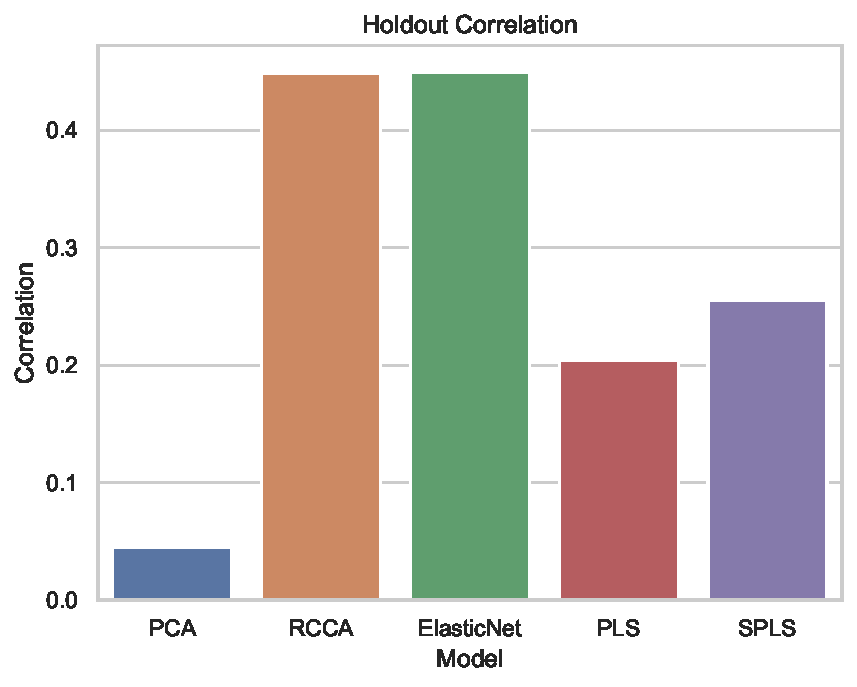
\includegraphics[width=0.5\linewidth]{figures/hcp/holdout_correlations}
    \caption{\textbf{HCP:} Out-of-sample canonical correlations for each model.}
\end{figure}

Nonetheless, the Elastic Net model did produce sparser weights than the Ridge CCA model (Figure~\ref{fig:sparsity}) with the Elastic Net model using 241 and 96 non-zero weights for the brain and behaviour views respectively.
This is compared to 300 and 145 non-zero weights for the brain and behaviour views respectively for the Ridge CCA model.
The SPLS model used even fewer variables with 118 and 56 non-zero weights for the brain and behaviour views respectively.
Given that the Elastic Net model can produce the same performance as the Ridge CCA model with fewer variables, we might then be inclined to prefer the Elastic Net model.

\begin{table}[h]
    \centering
    \caption{\textbf{HCP:} Number of non-zero \gls{weights} for each model.}
    \begin{tabular}{|c|c|c|}
        \hline
        Model       & Brain Weights & Behaviour Weights \\
        \hline
        PCA         & 300           & 145               \\
        RCCA        & 300           & 145               \\
        Elastic Net & 241           & 96                \\
        PLS         & 300           & 145               \\
        SPLS        & 118           & 56                \\
        \hline
    \end{tabular}\label{tab:brain-behaviour-weights-hcp}
\end{table}

\subsubsection{Behaviour Weights}

Figure\ref{fig:behaviour} plots the top 8 positive and negative non-imaging \gls{weights} for each model.
This is to illustrate some of the effects we have observed in the previous section.
PCA finds a mode of variation in the behavioural data that is positively correlated with psychiatric and life function tests and negatively correlated with a number of emotion and personality tests.
The RCCA and Elastic Net models find a mode of variation in the behavioural data that is negatively correlated with the Line Orientation test and to a lesser extent smoking and positively correlated with a number of other cognitive tests.
The PLS model finds a mode of variation in the behavioural data that is somewhat similar to the `positive-negative' mode in \citet{smith2015positive} with a positive correlation with agreeableness, vocabulary tests, and feelings about ones' life and a strong negative correlation with smoking, rule-breaking, and antisocial personality traits.
The SPLS mode is similar but selects out the rule-breaking and antisocial personality traits in favour of the vocabulary tests and smoking. This appears consistent with the additional preprocessing steps in \citet{smith2015positive}, which included a top-100 PCA projection of both the brain and behaviour data.

\begin{figure}[h]
    \centering
    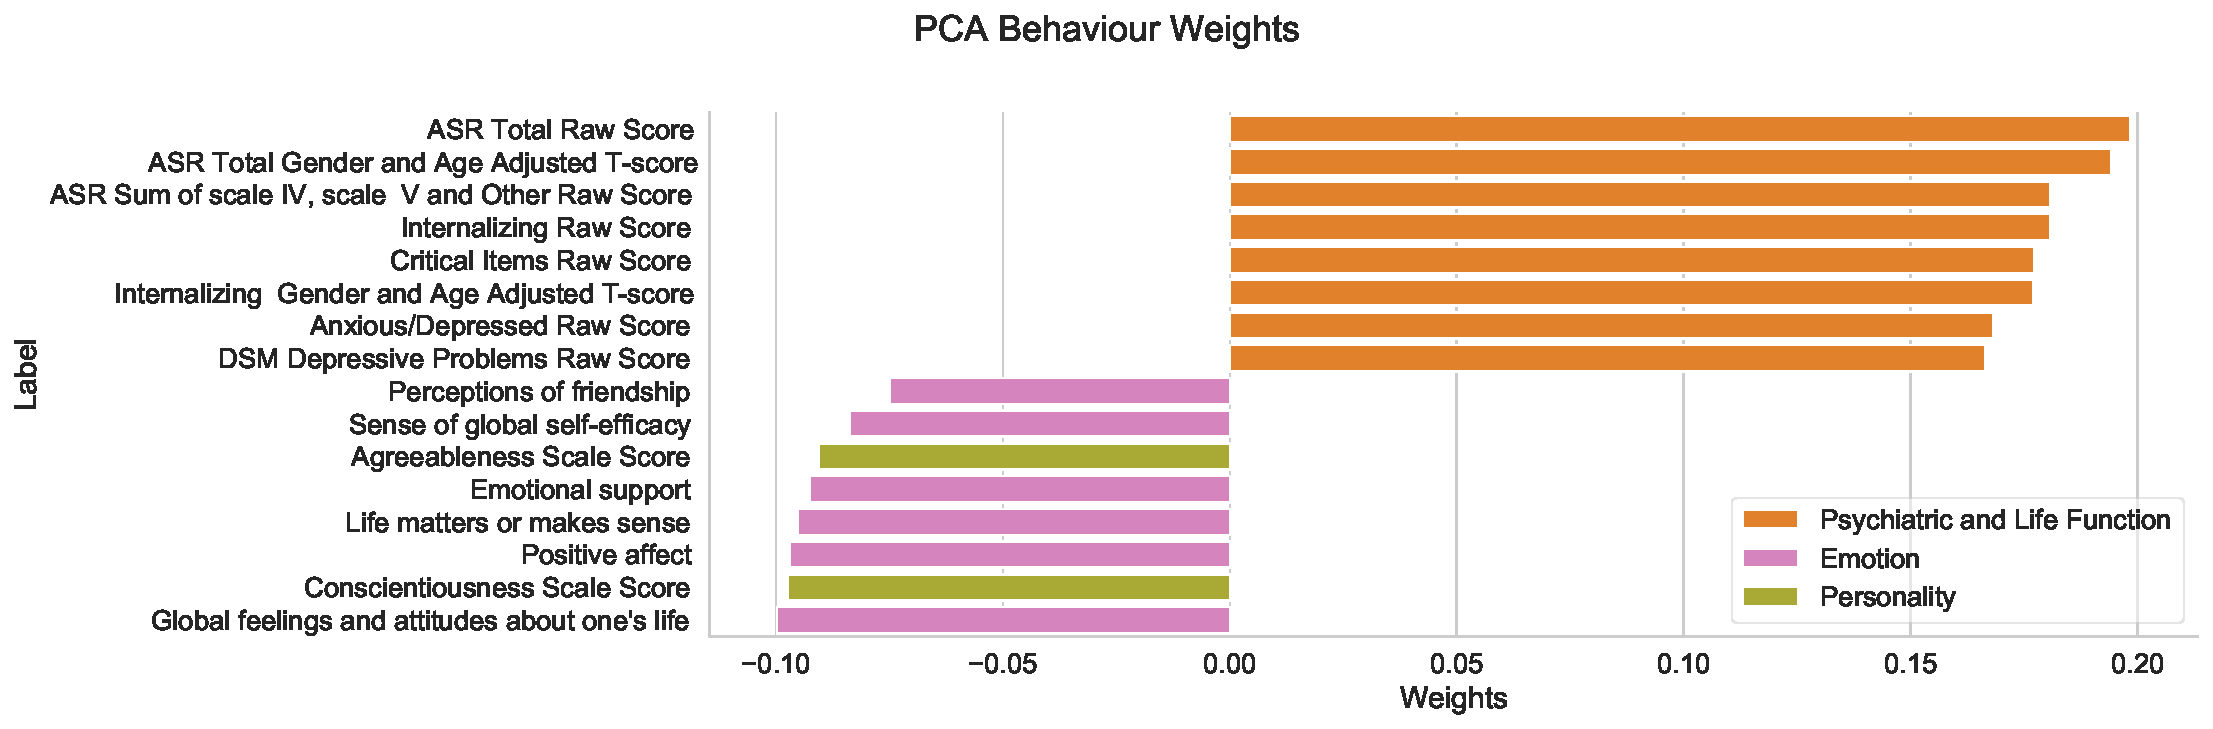
\includegraphics[width=0.8\linewidth]{figures/hcp/PCA behaviour weights}
    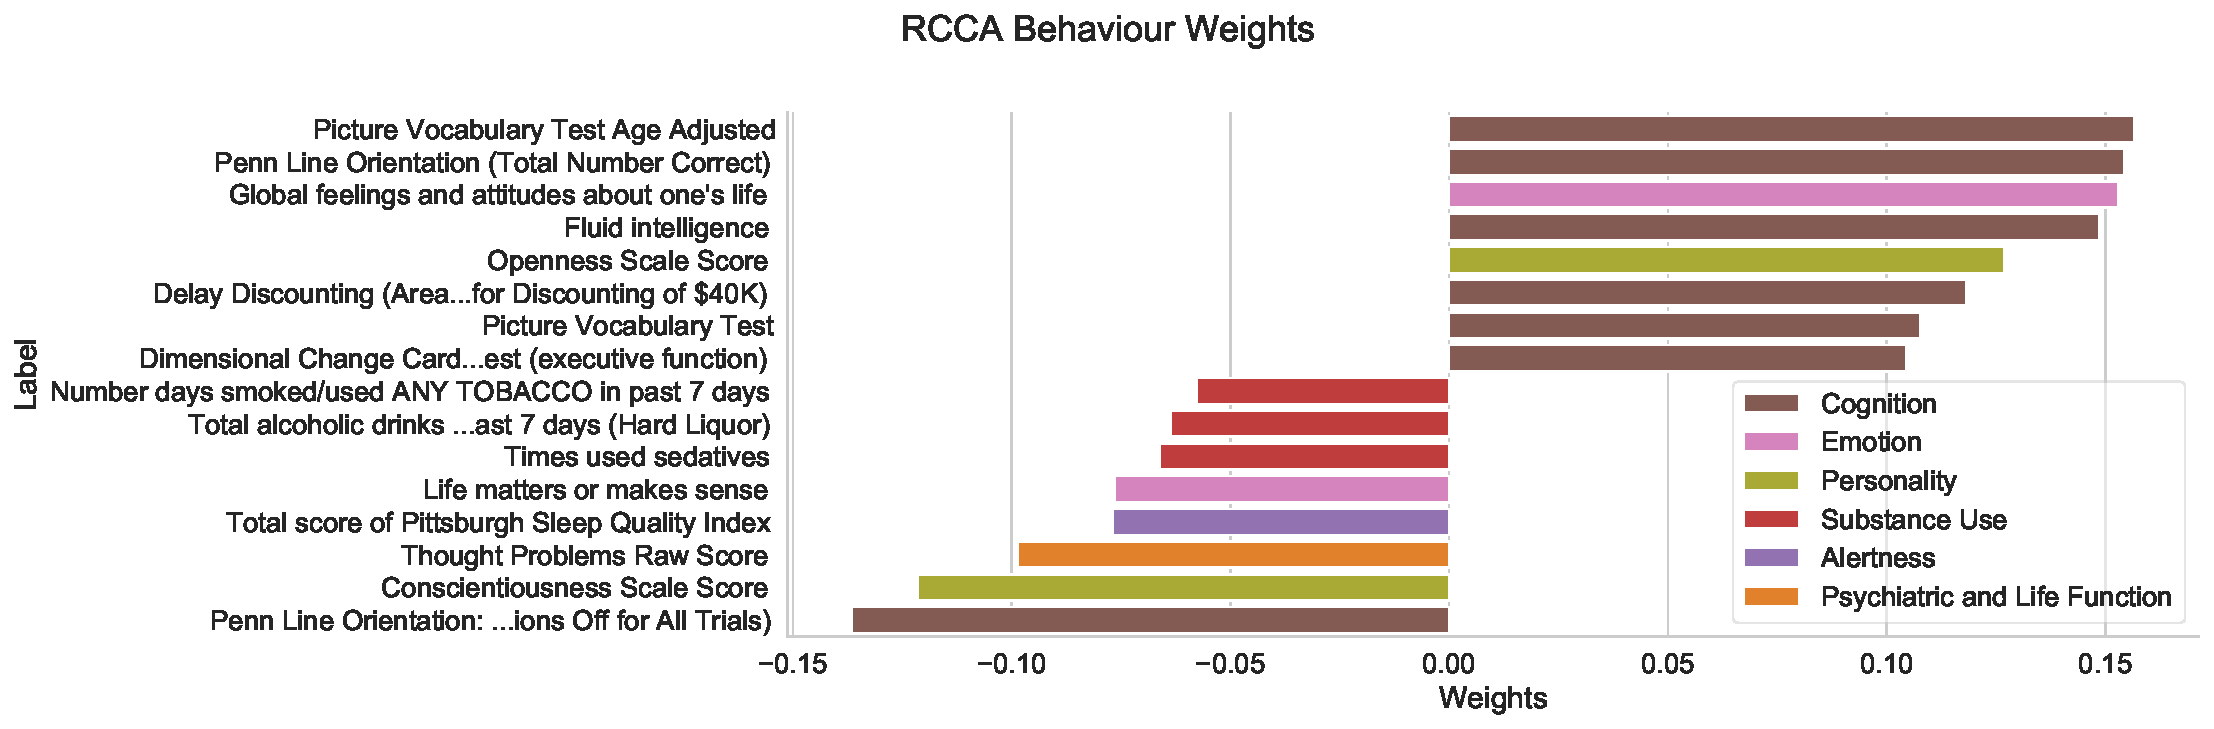
\includegraphics[width=0.8\linewidth]{figures/hcp/RCCA behaviour weights}
    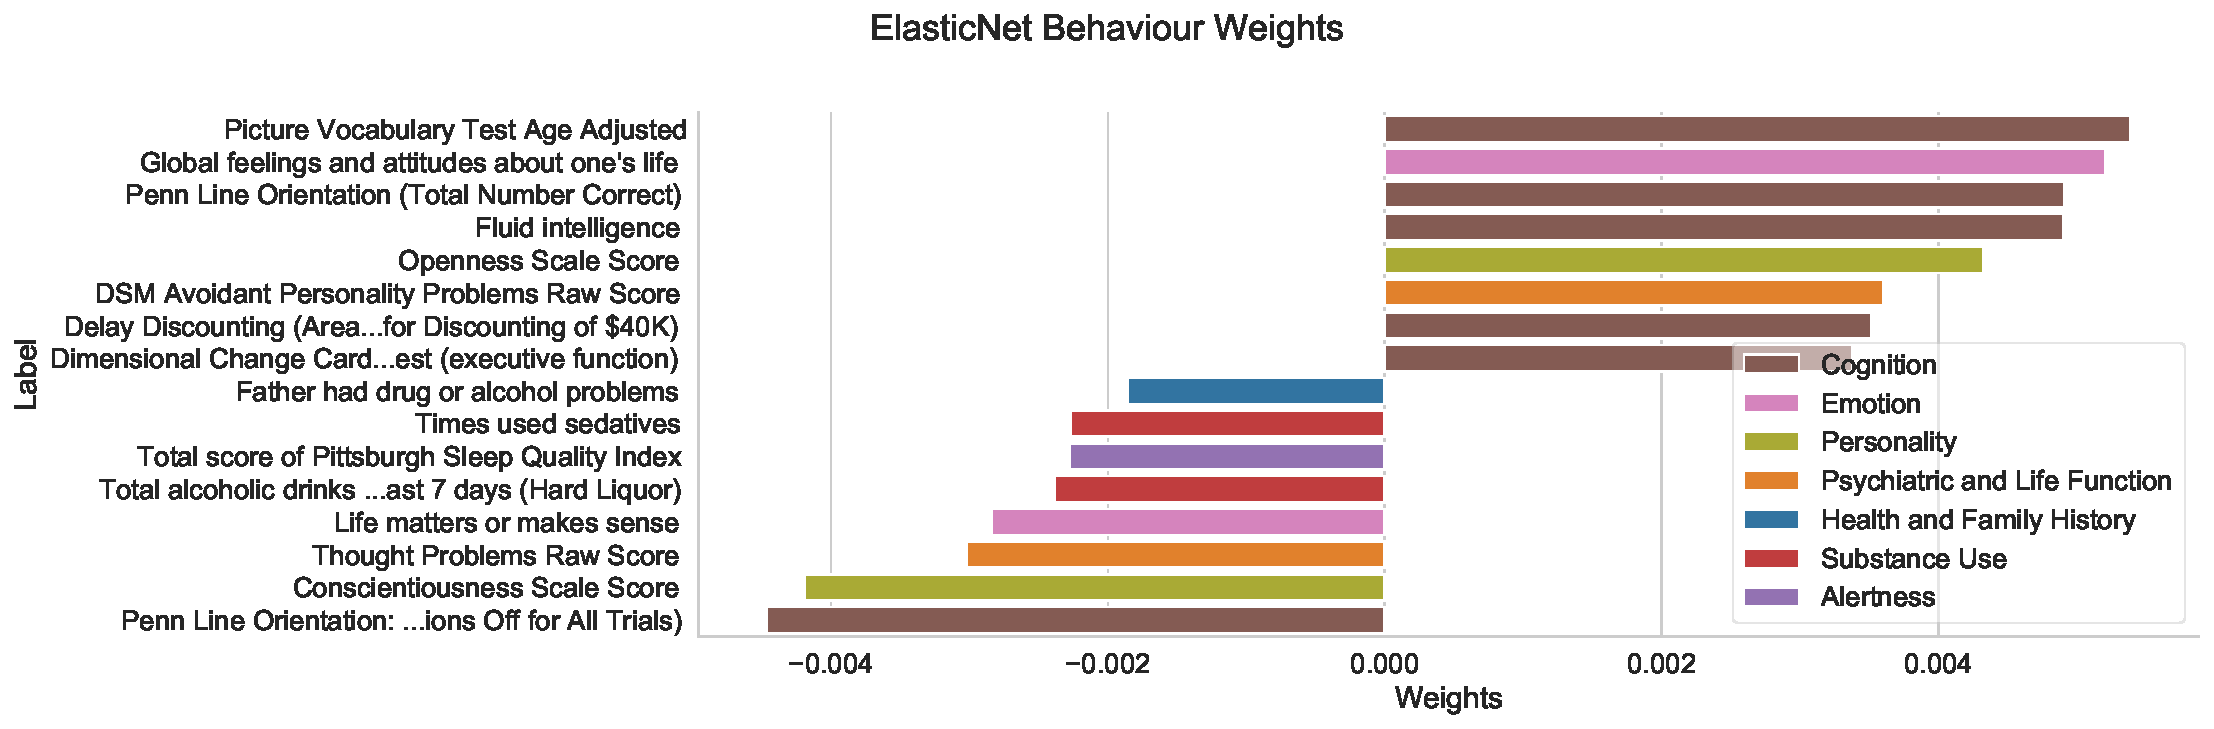
\includegraphics[width=0.8\linewidth]{figures/hcp/ElasticNet behaviour weights}
    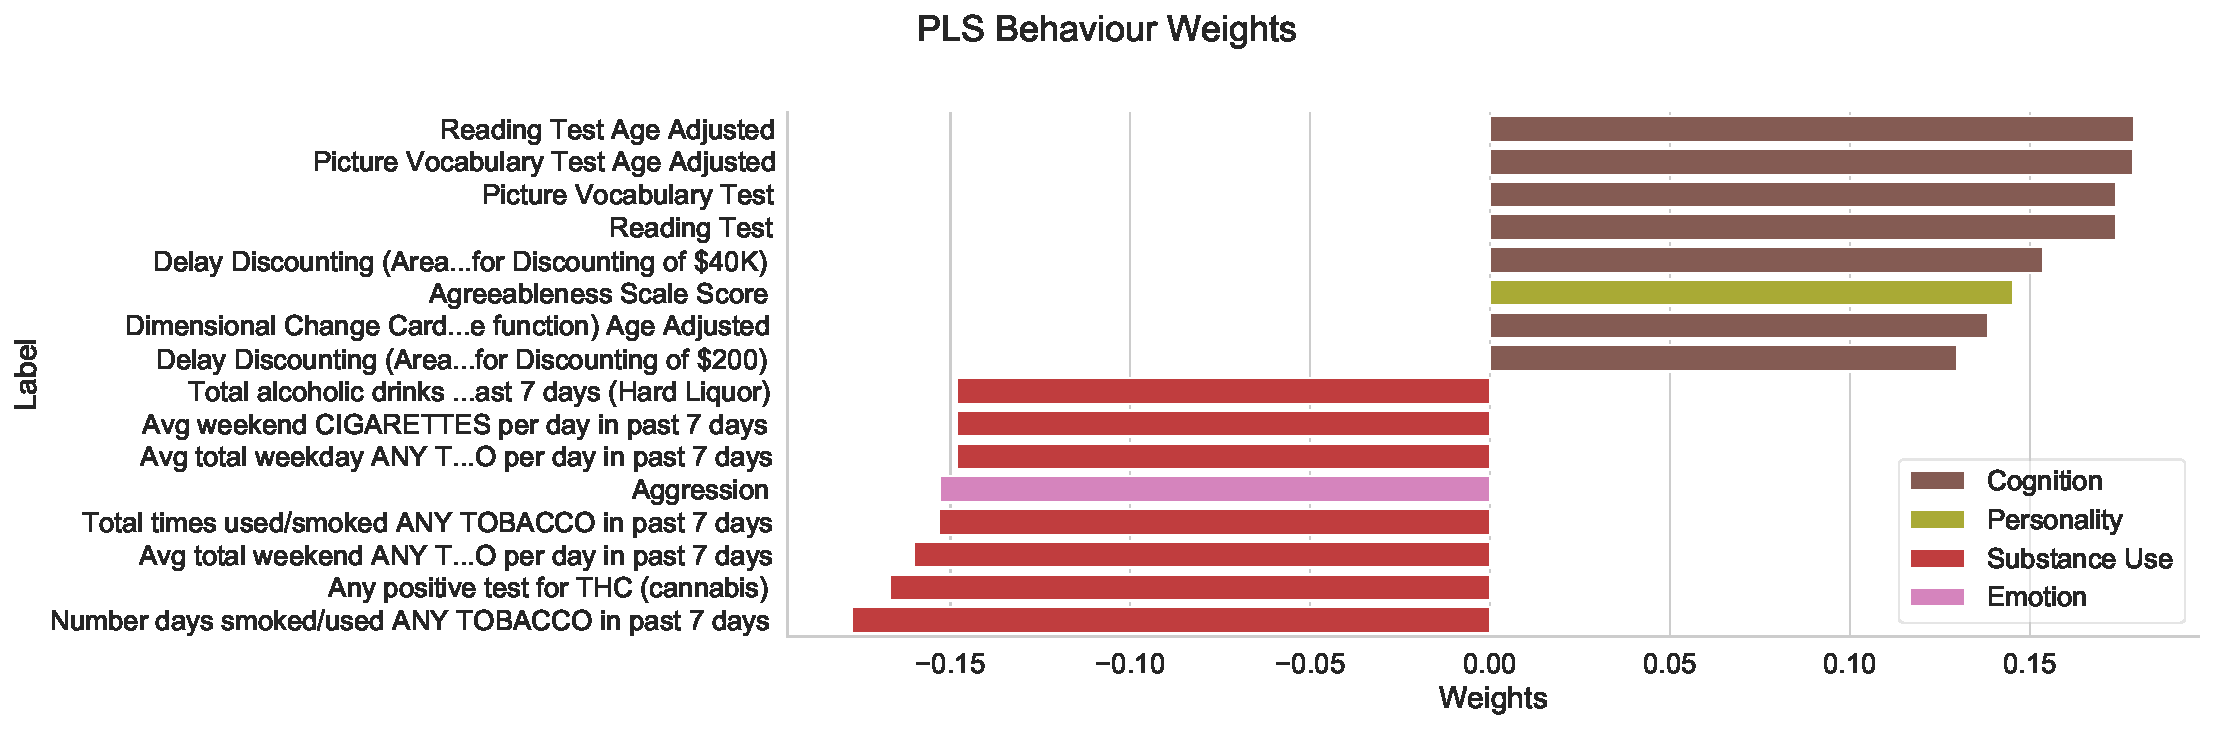
\includegraphics[width=0.8\linewidth]{figures/hcp/PLS behaviour weights}
    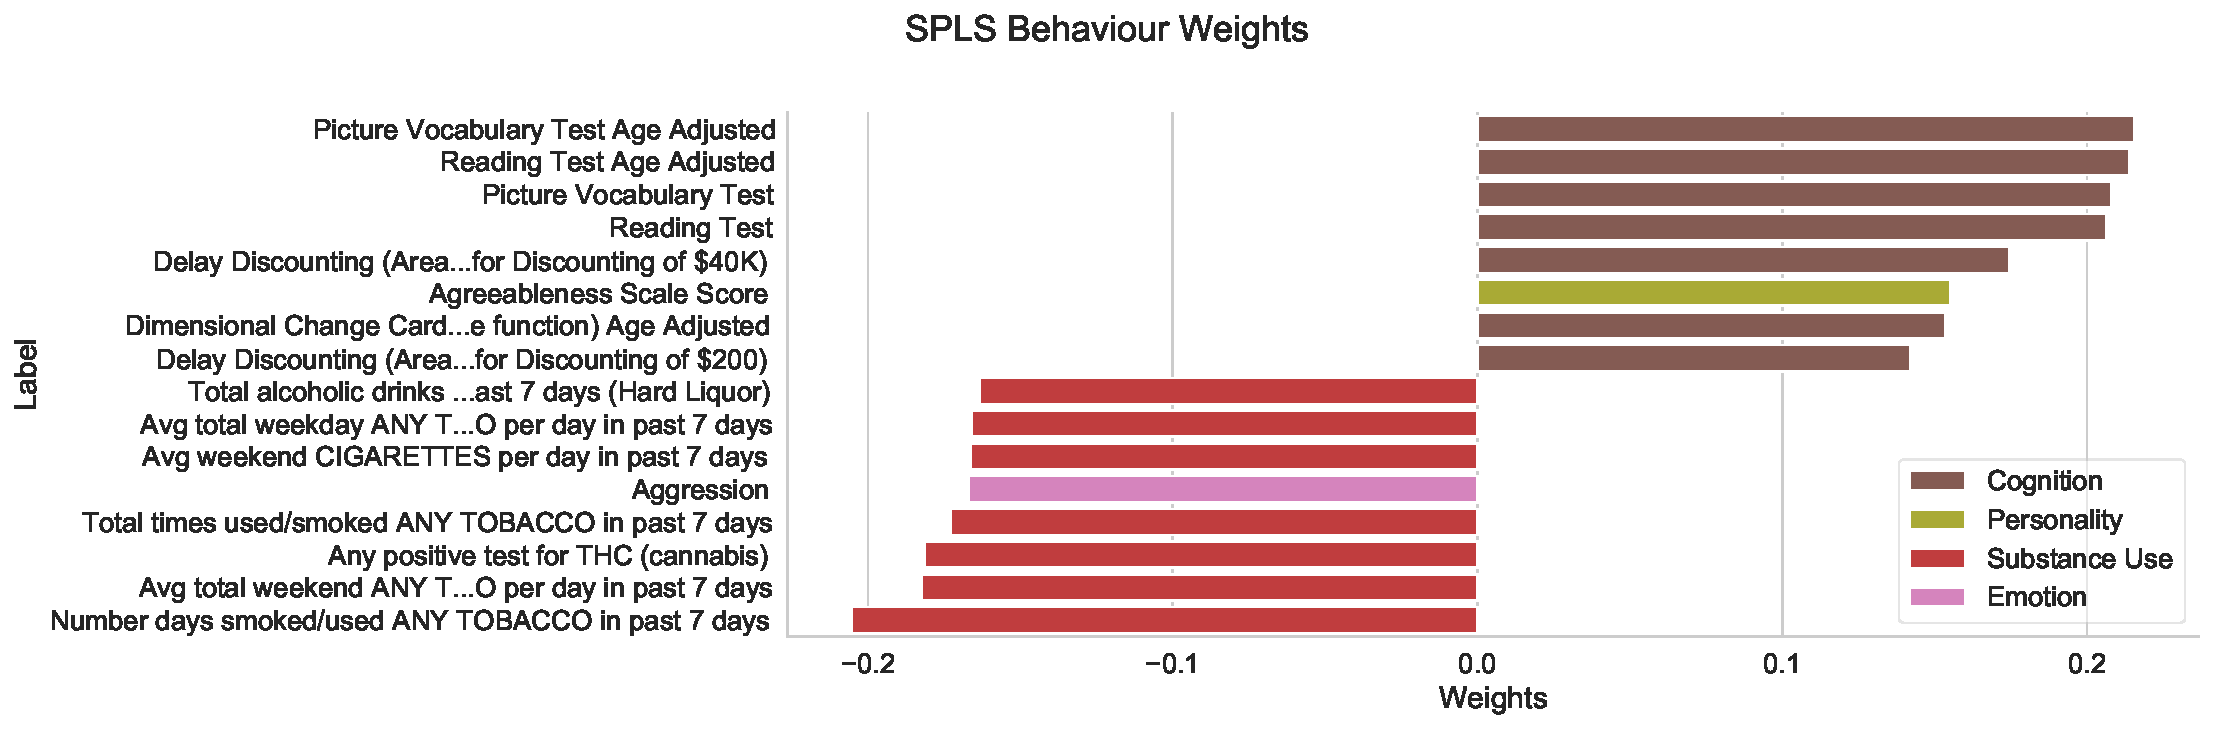
\includegraphics[width=0.8\linewidth]{figures/hcp/SPLS behaviour weights}
    \caption{\textbf{HCP:} Top 8 positive and negative non-imaging \gls{weights} for each model}\label{fig:behaviour}
\end{figure}

\subsubsection{Brain Connectivity Weights}

In this section, we use two different methods to visualize the brain connectivity weights.
The first method is to use chord diagrams to visualize the top 8 positive and negative brain \gls{weights} for each model.
This approach is inspired by the chord diagrams used in \cite{smith2015positive}.
The second method is to use surface maps to visualize the brain connectivity weights.
This approach has been used by both \cite{ferreira2022hierarchical} and \cite{smith2015positive}.

\paragraph{Chord Diagrams}
We grouped the nodes of the connectivity matrix of our data into 7 parcels according to the Yeo 7 network parcellation \cite{yeo2011organization}.
This was achieved by assigning each node to the network with the highest voxelwise overlap.
These are then arranged around the circumference of the chord diagram using the Nichord package \citep{bogdan2023connsearch}.
The plots then show the 8 strongest positive and negative \gls{weights} for each model as `chords'.
The chord diagrams in Figure~\ref{fig:chord_weights} show the top 8 positive and negative brain \gls{weights} for each model.

\begin{itemize}
    \item The \textbf{RCCA} model displays a diverse set of connections across all networks, with especially prominent weights in the \textcolor{red}{somatomotor} and \textcolor{blue}{default mode} networks.

    \item The \textbf{ElasticNet} model presents similar connections between the \textcolor{red}{somatomotor} and \textcolor{blue}{default mode} networks.

    \item The \textbf{PLS} model exhibits strong connections between the \textcolor{green}{frontoparietal} and \textcolor{pink}{visual} networks.

    \item The \textbf{SPLS} model exhibits similar connections between the \textcolor{green}{frontoparietal} and \textcolor{pink}{visual} networks.
\end{itemize}

This is perhaps consistent with the behaviour data as the somatomotor network is associated with motor function and sensory processing which is related to the Line Orientation test, requiring spatial reasoning and motor coordination.

The correlations made by the PLS and SPLS models between substance abuse and cognitive tests could be due to the significant role the frontoparietal network plays in executive function, which can be impaired by substance abuse.
Likewise, the visual network is likely involved in a number of the cognitive tests and could be disrupted by substance abuse.

The RCCA and ElasticNet models might be detecting more integrative and possibly higher cognitive functions, while the PLS and SPLS models might be highlighting the more immediate cognitive processes that can be disrupted by substance abuse.

\begin{figure}[h]
    \centering
    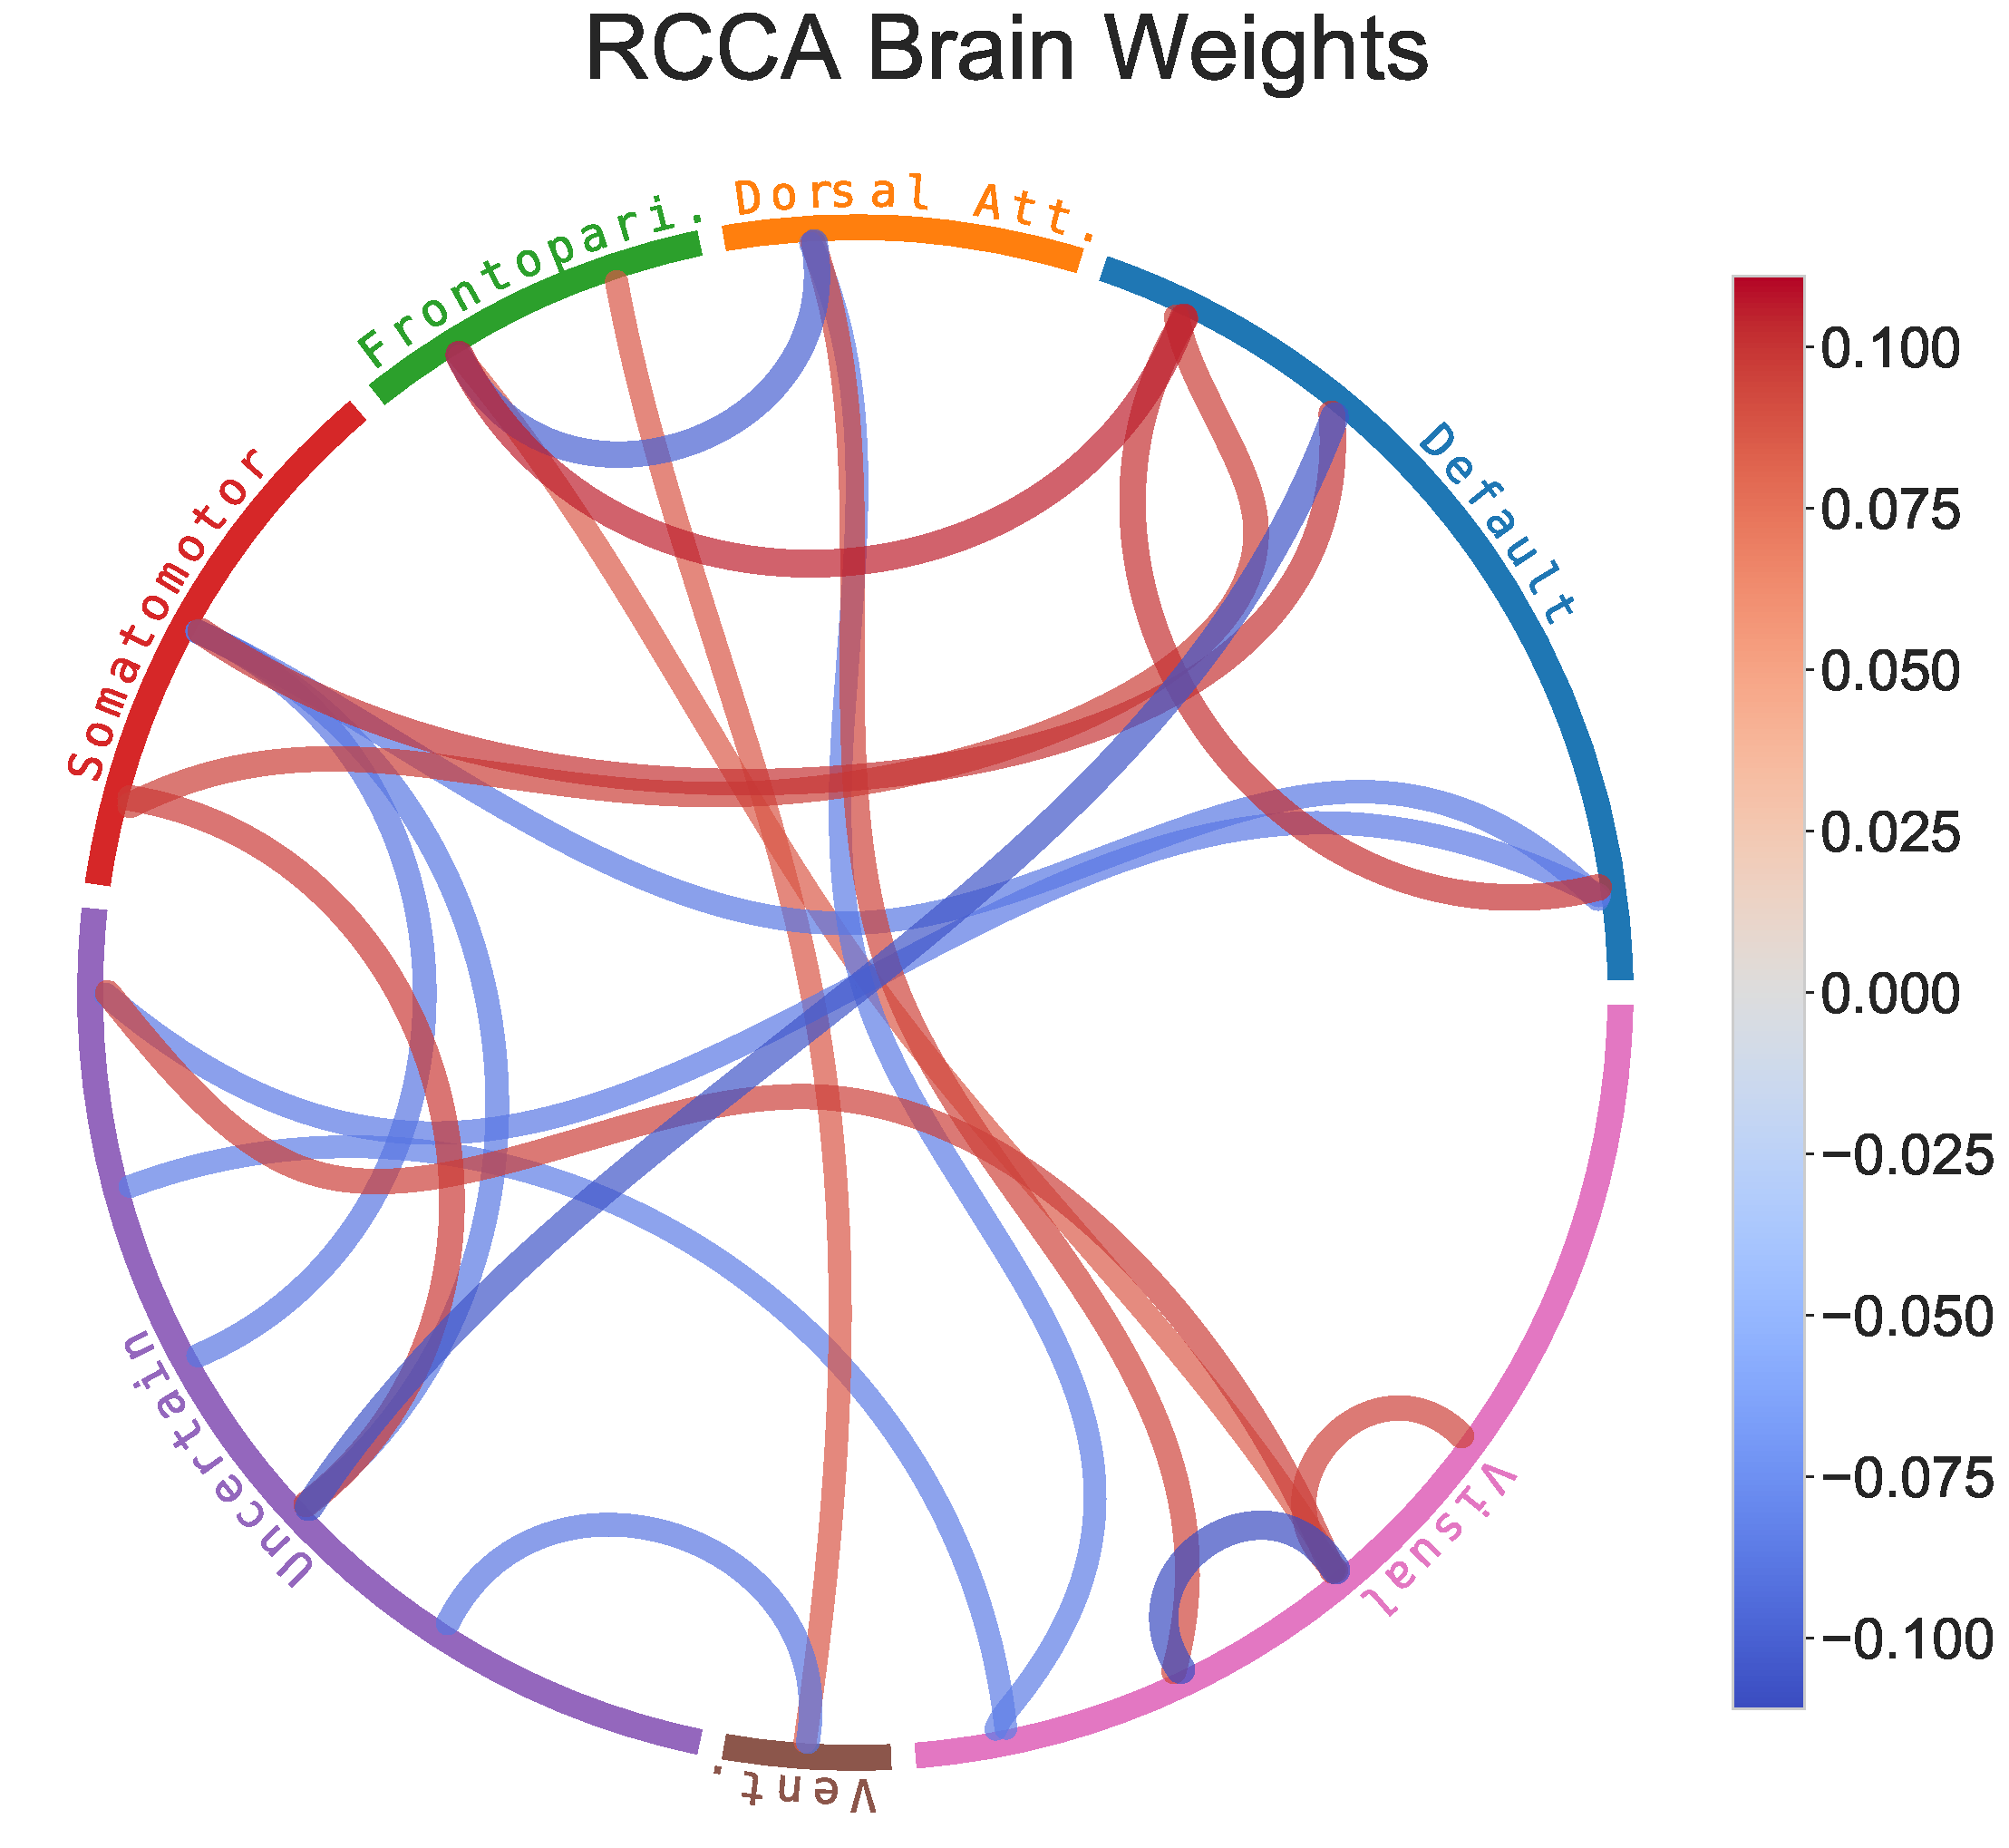
\includegraphics[width=0.49\linewidth]{figures/hcp/RCCA brain weights}
    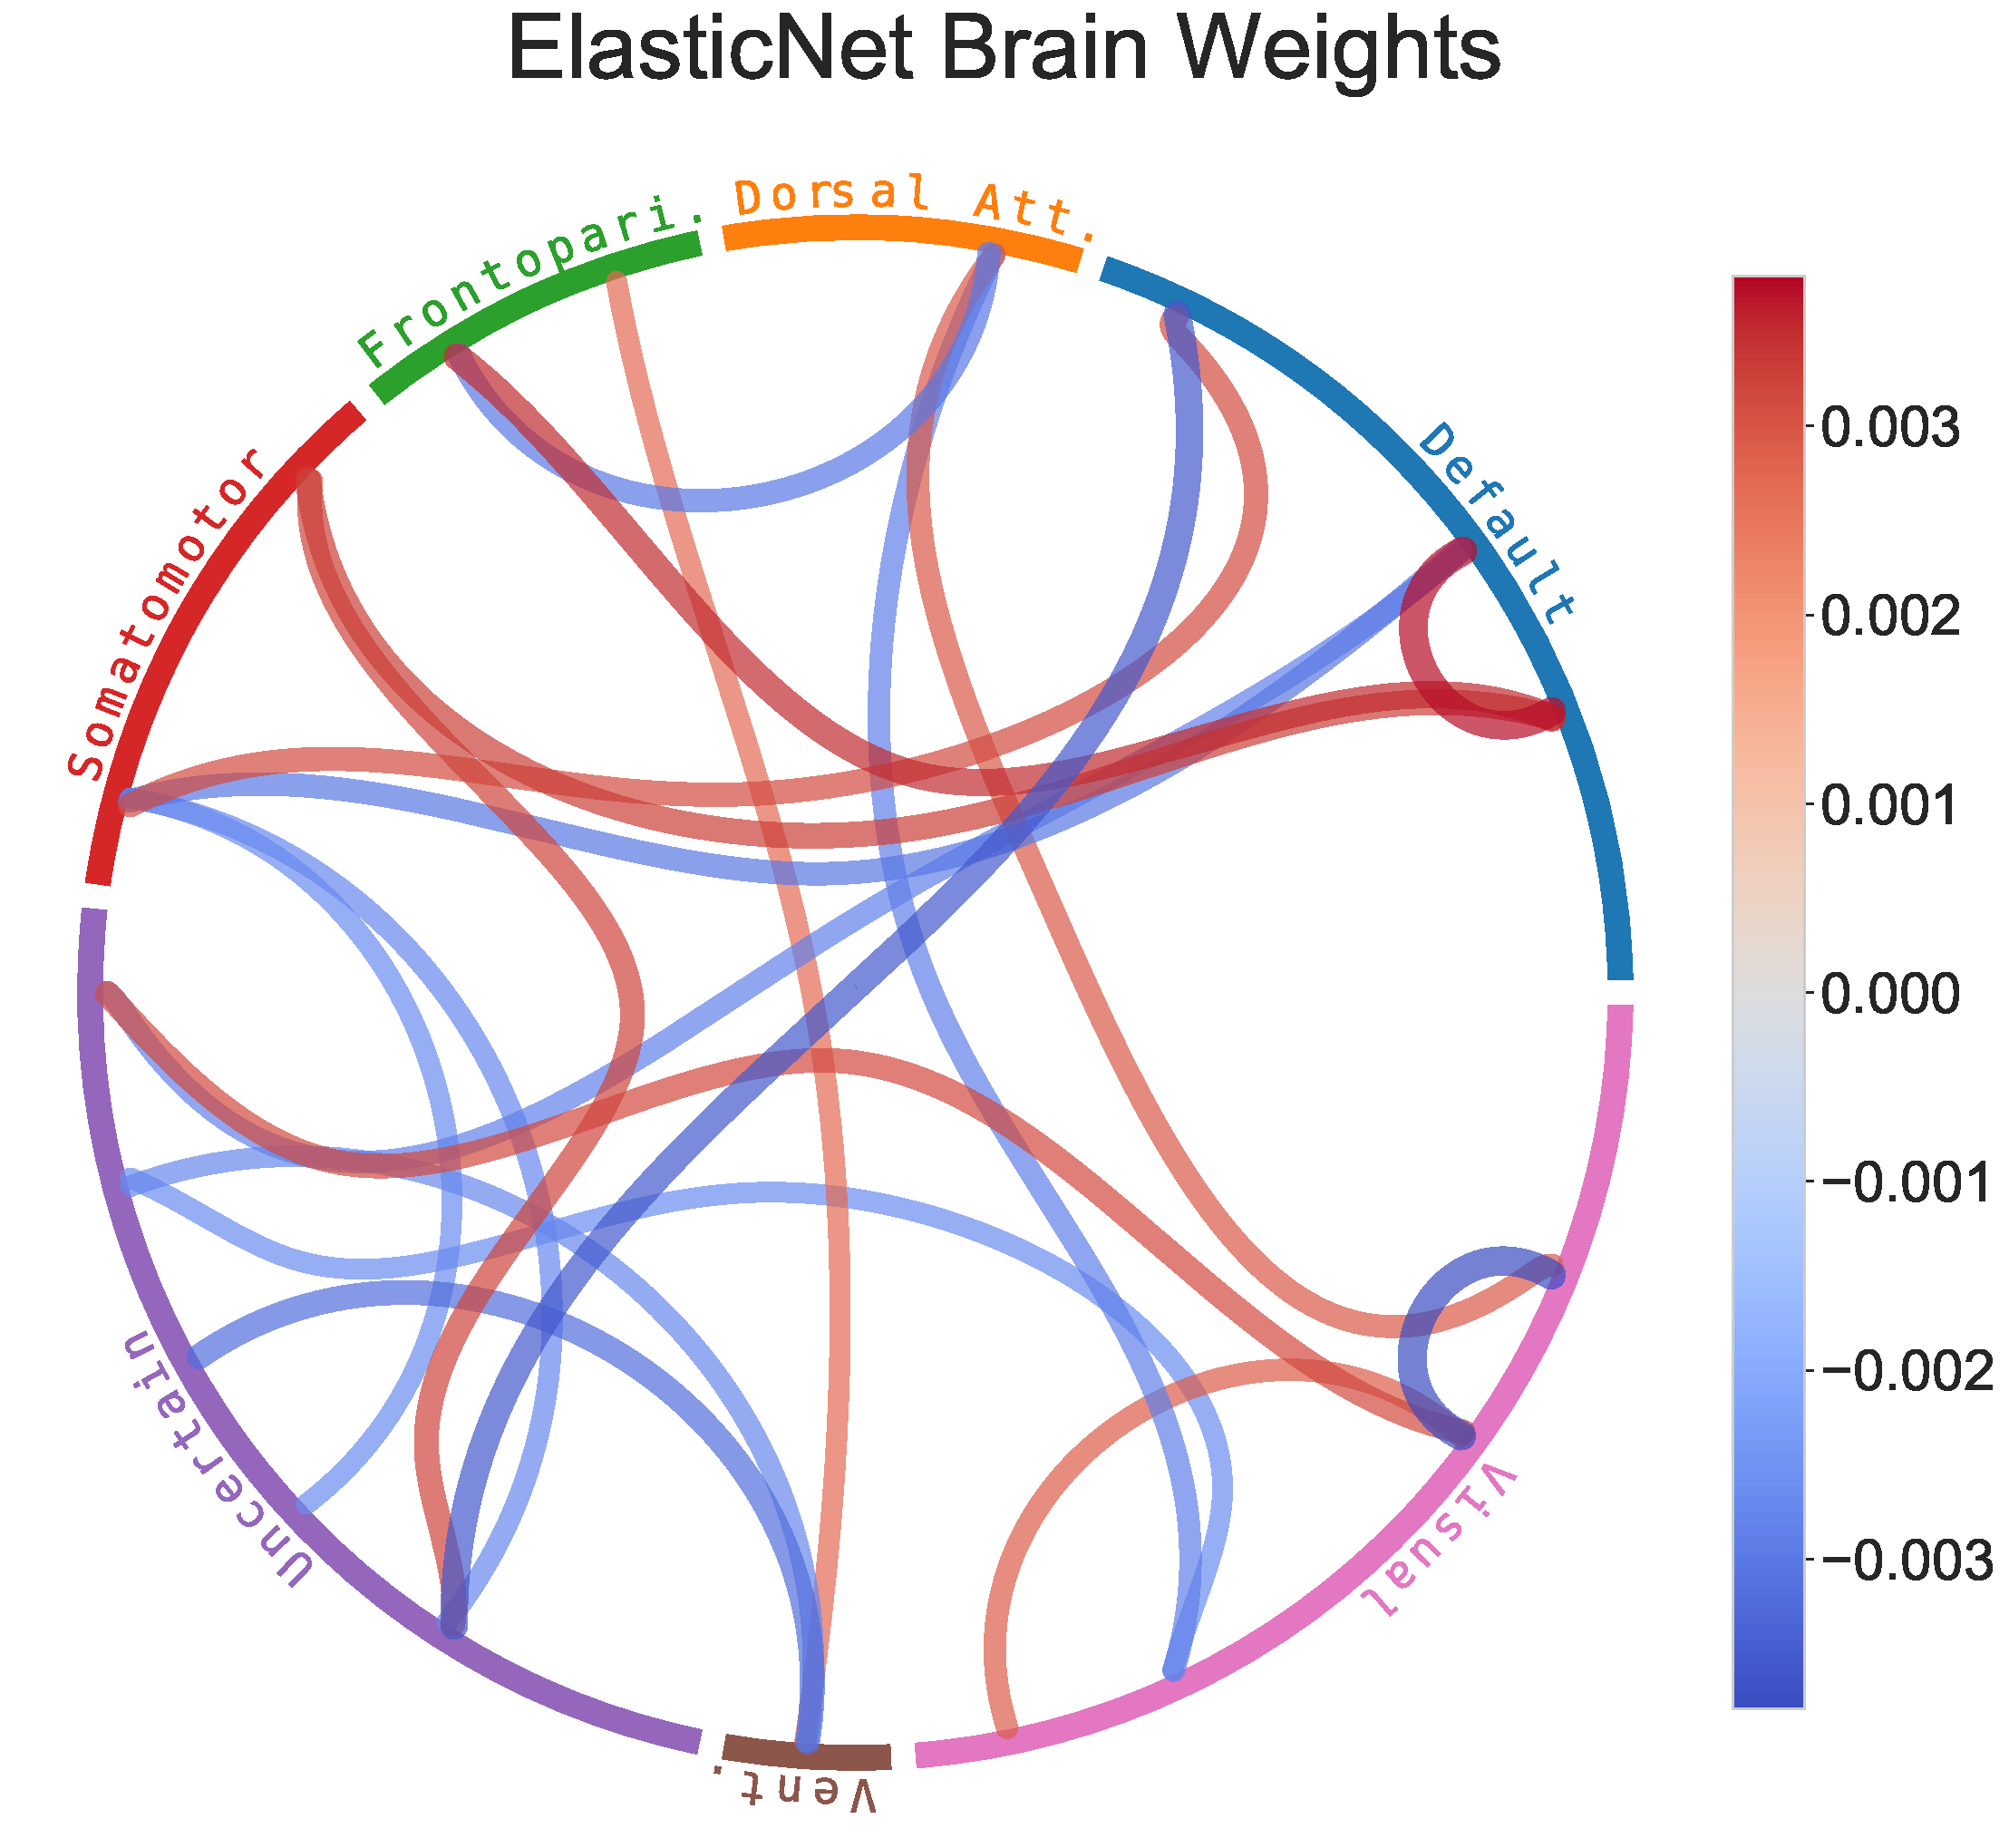
\includegraphics[width=0.49\linewidth]{figures/hcp/ElasticNet brain weights}
    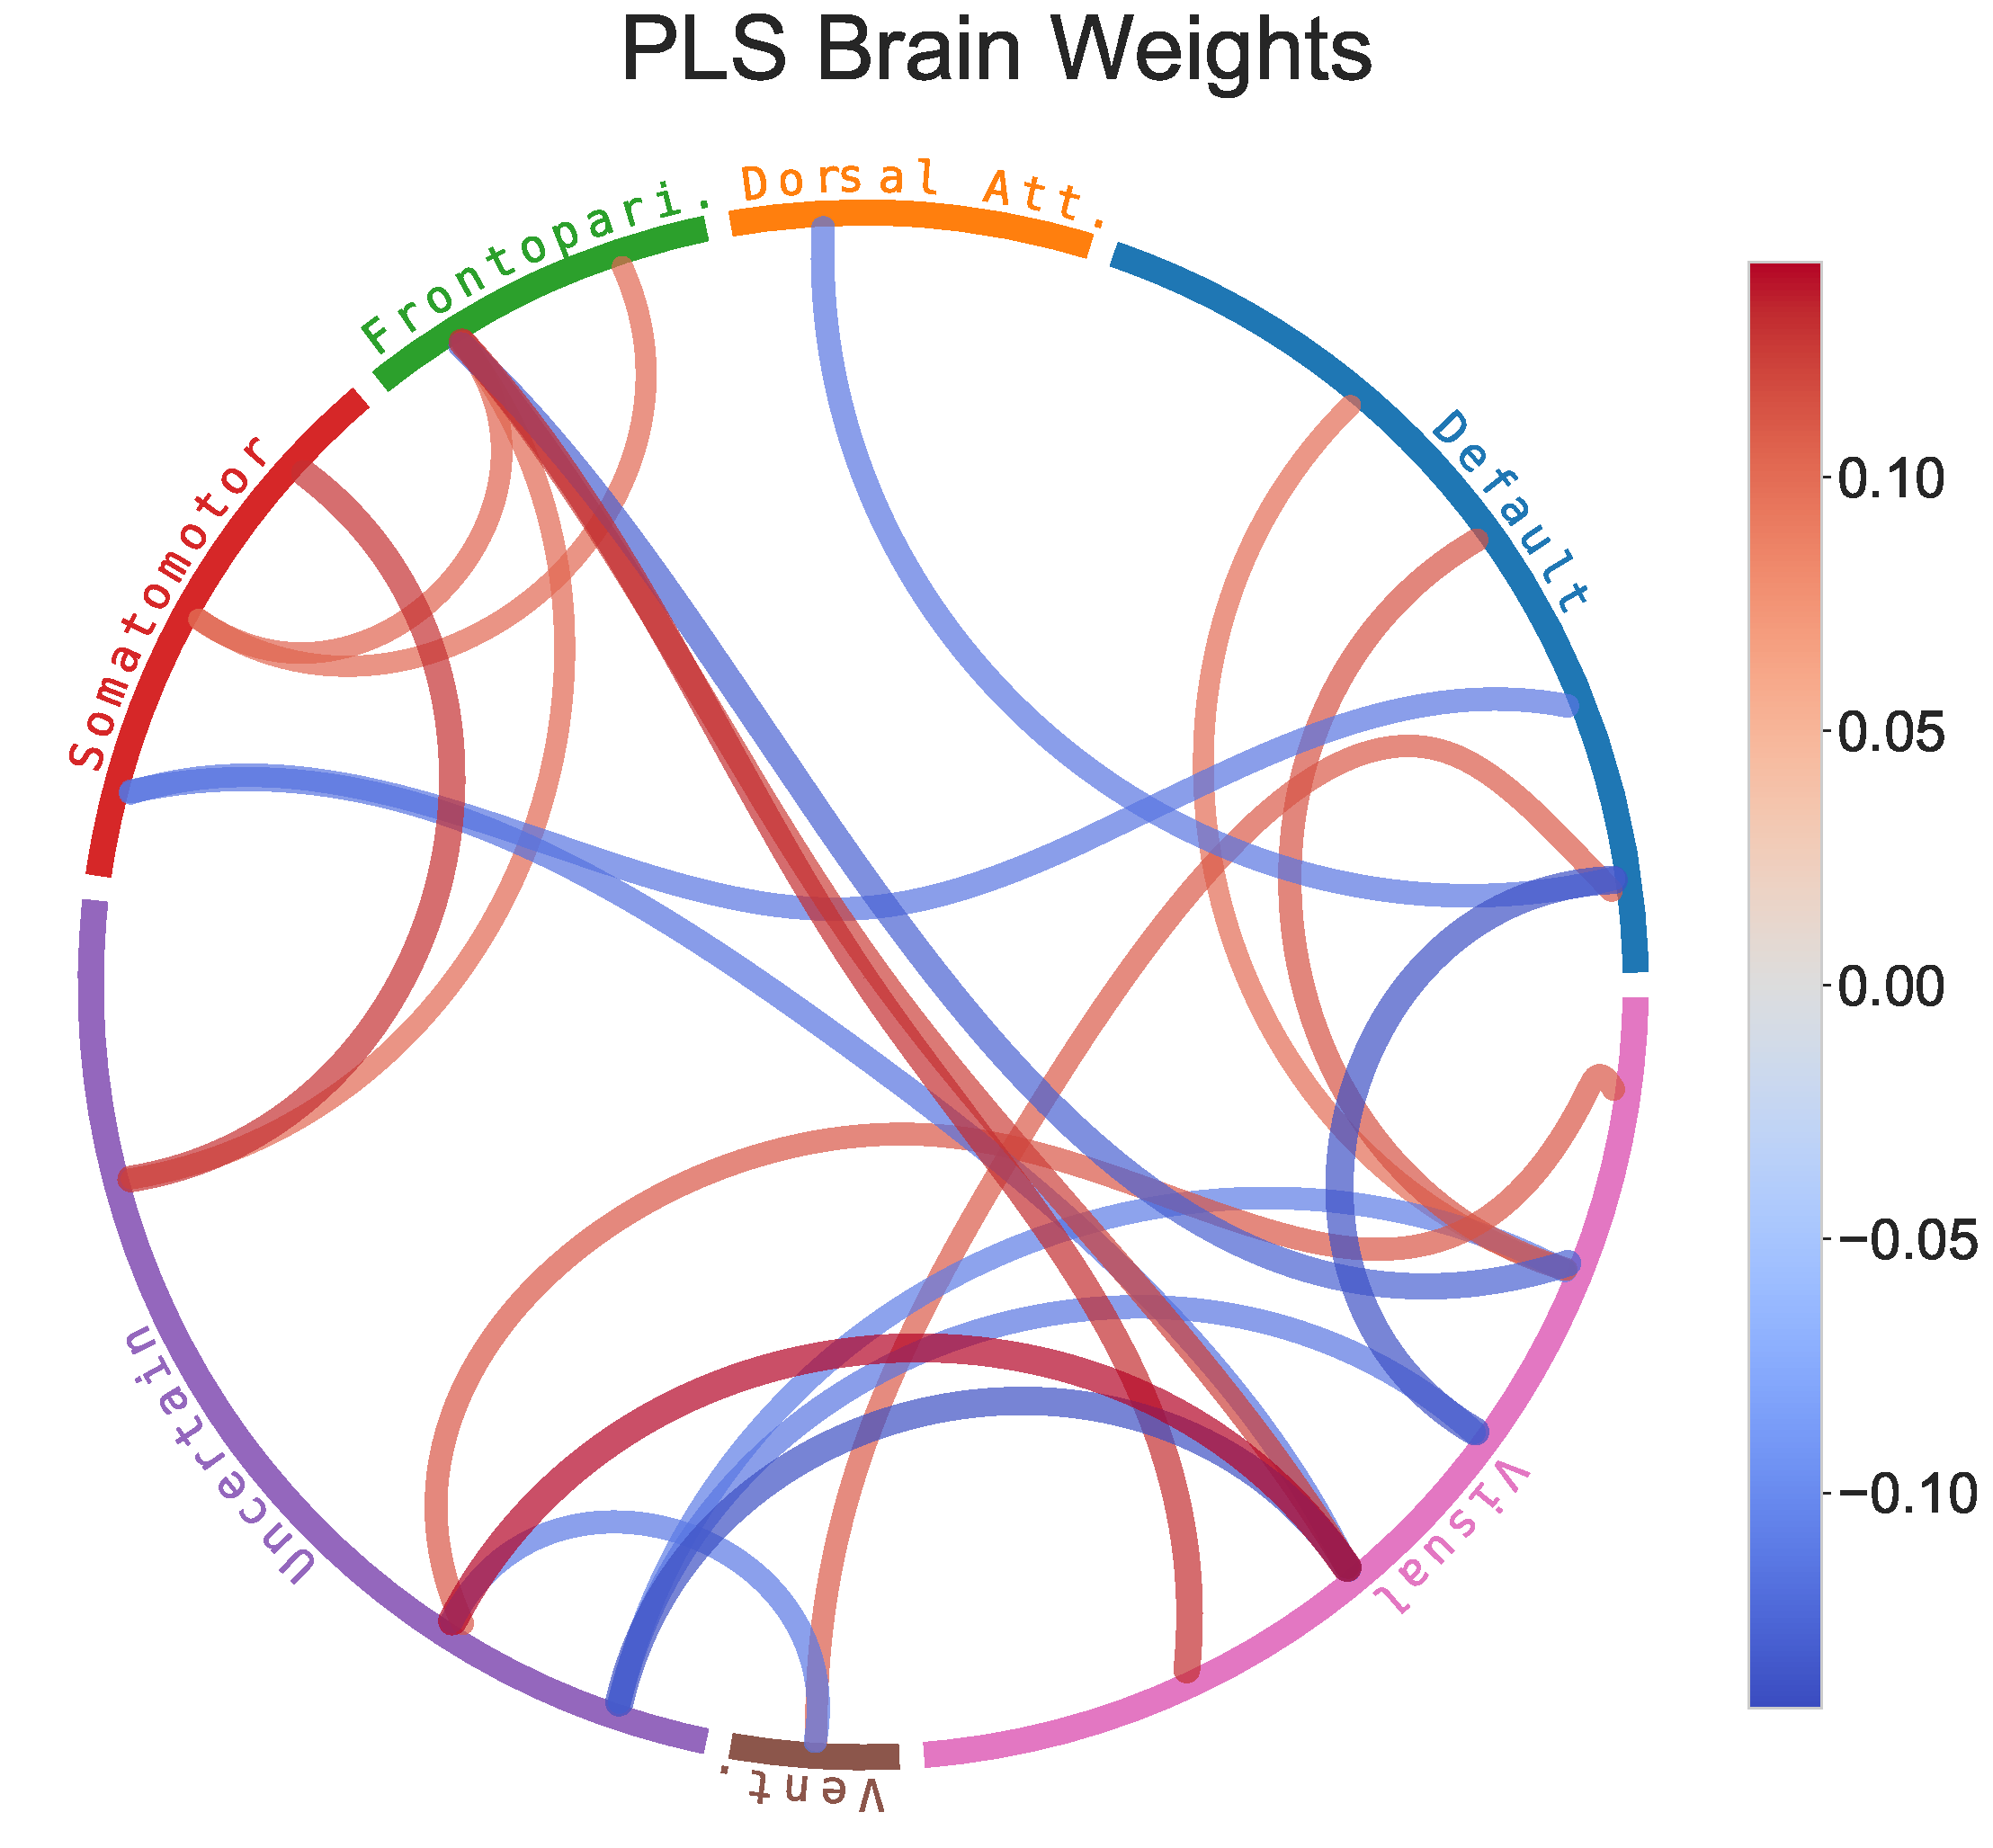
\includegraphics[width=0.49\linewidth]{figures/hcp/PLS brain weights}
    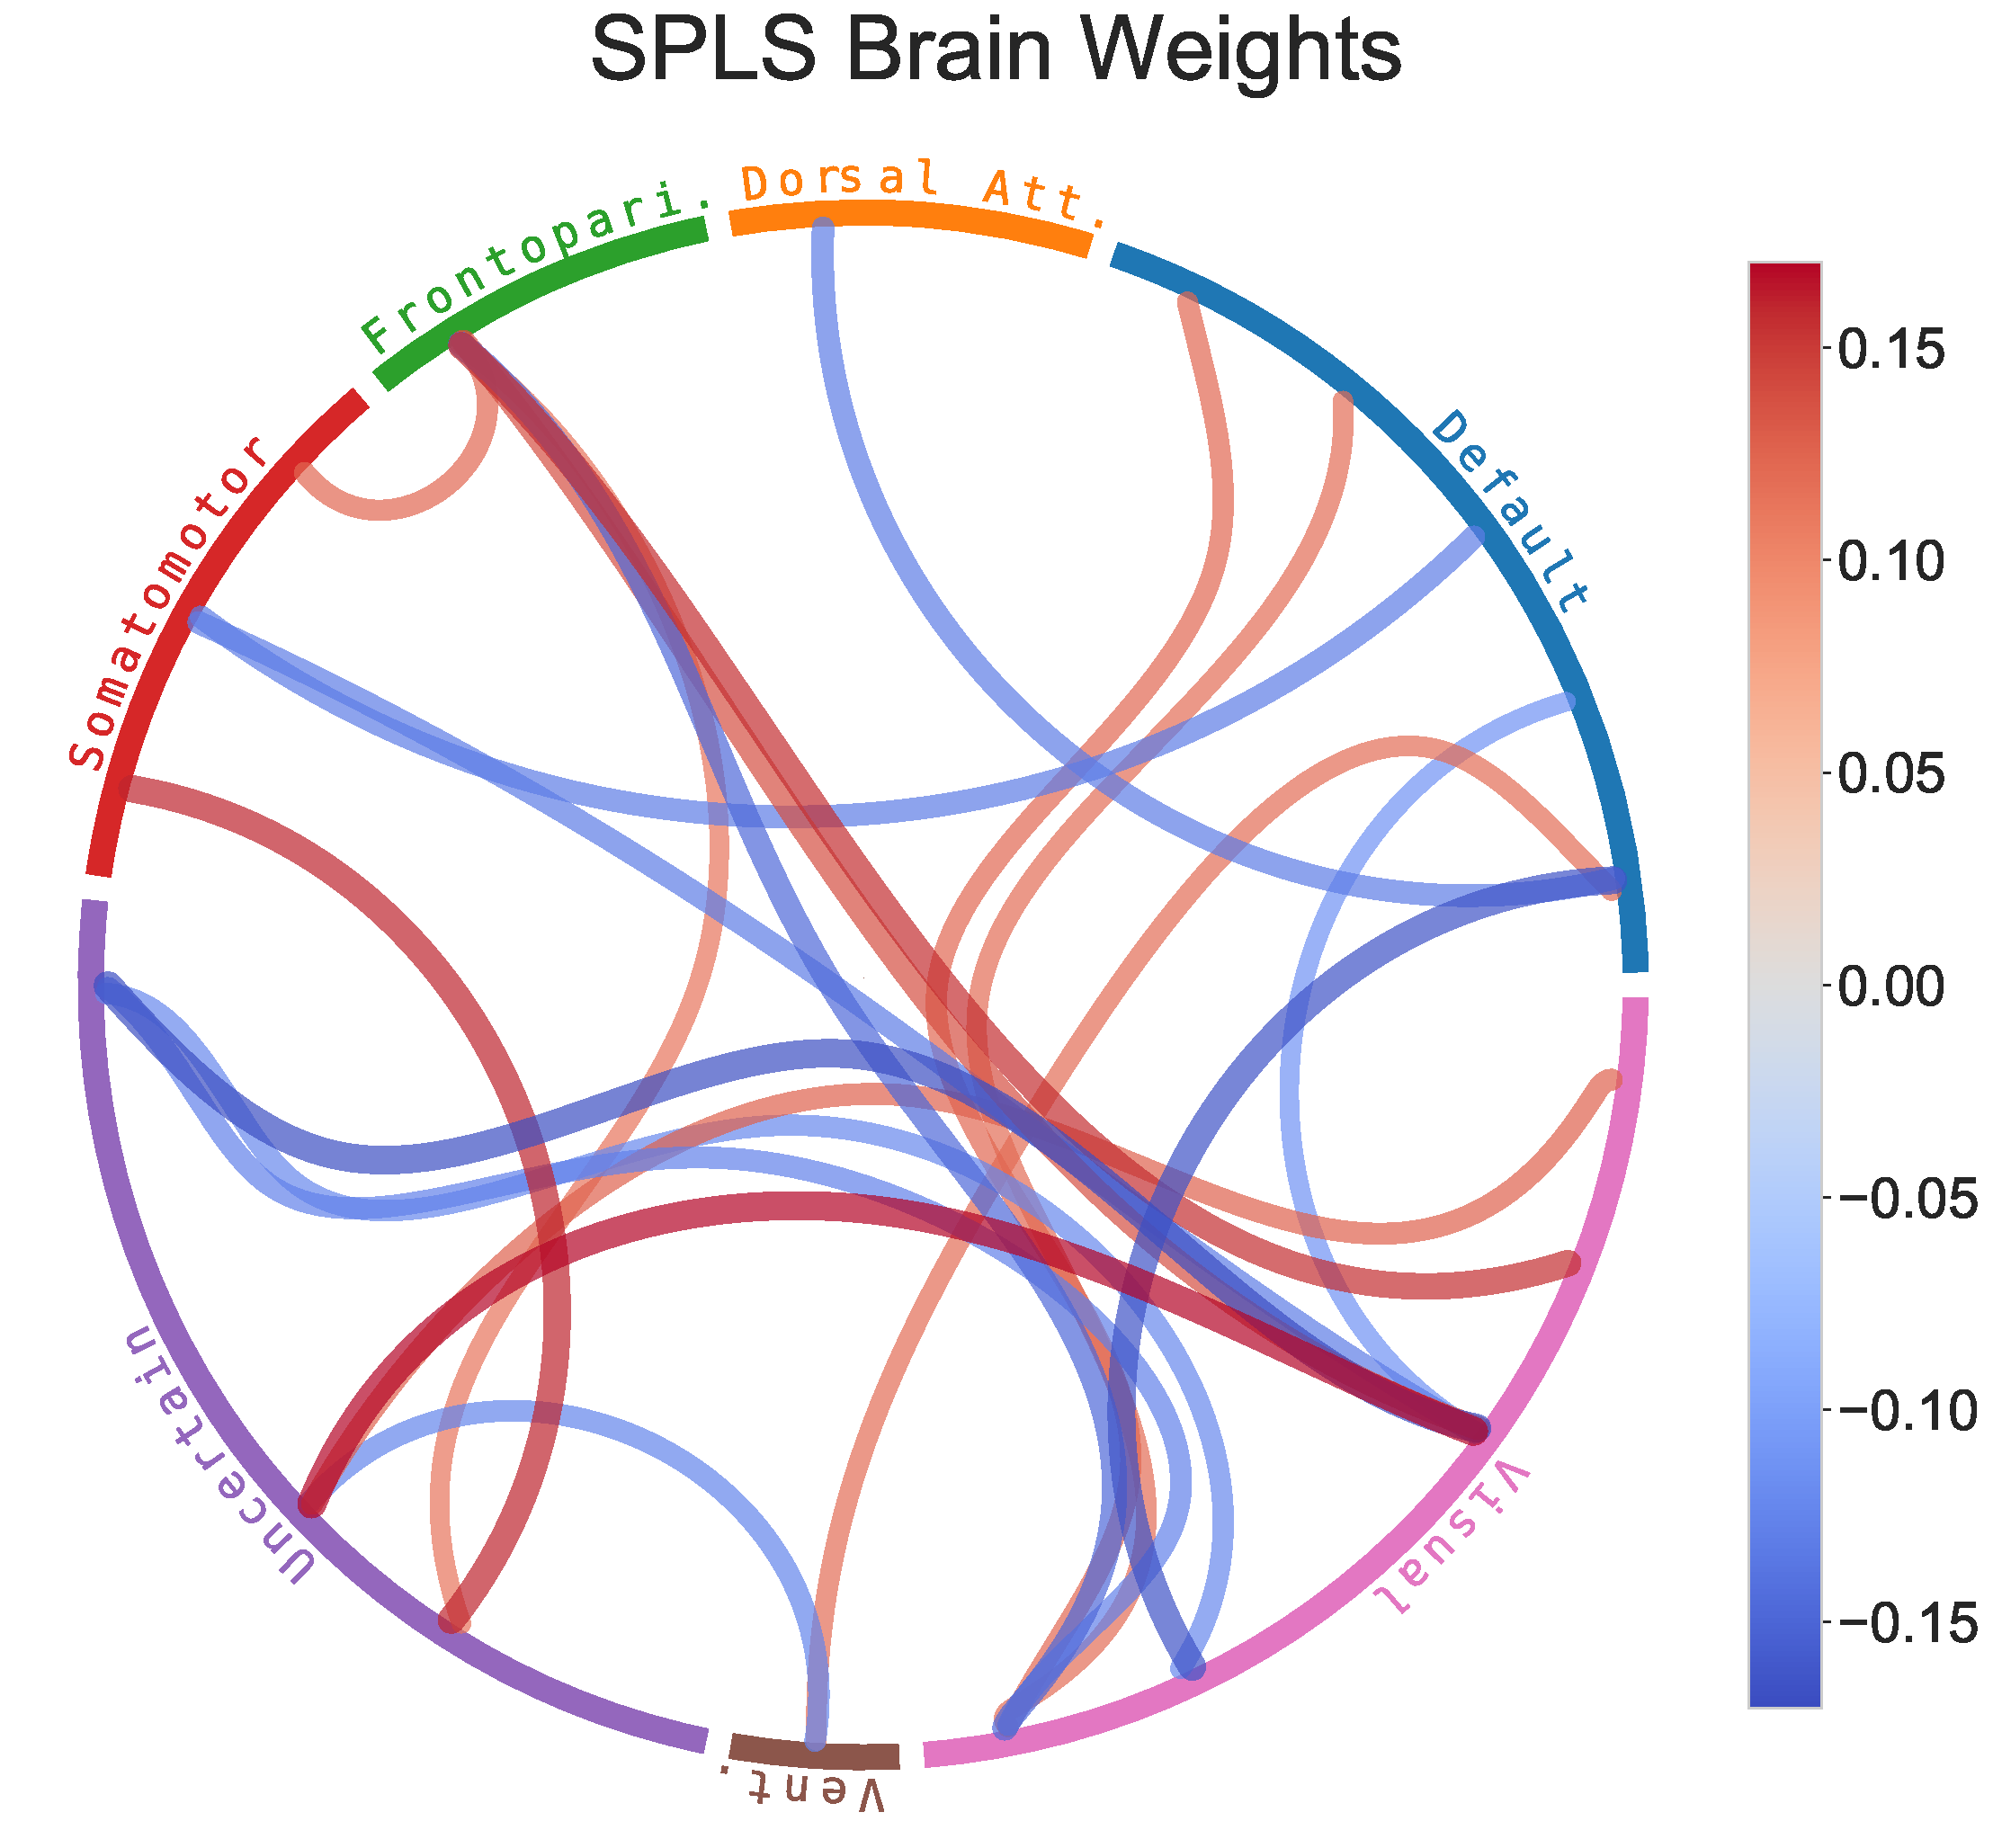
\includegraphics[width=0.49\linewidth]{figures/hcp/SPLS brain weights}
    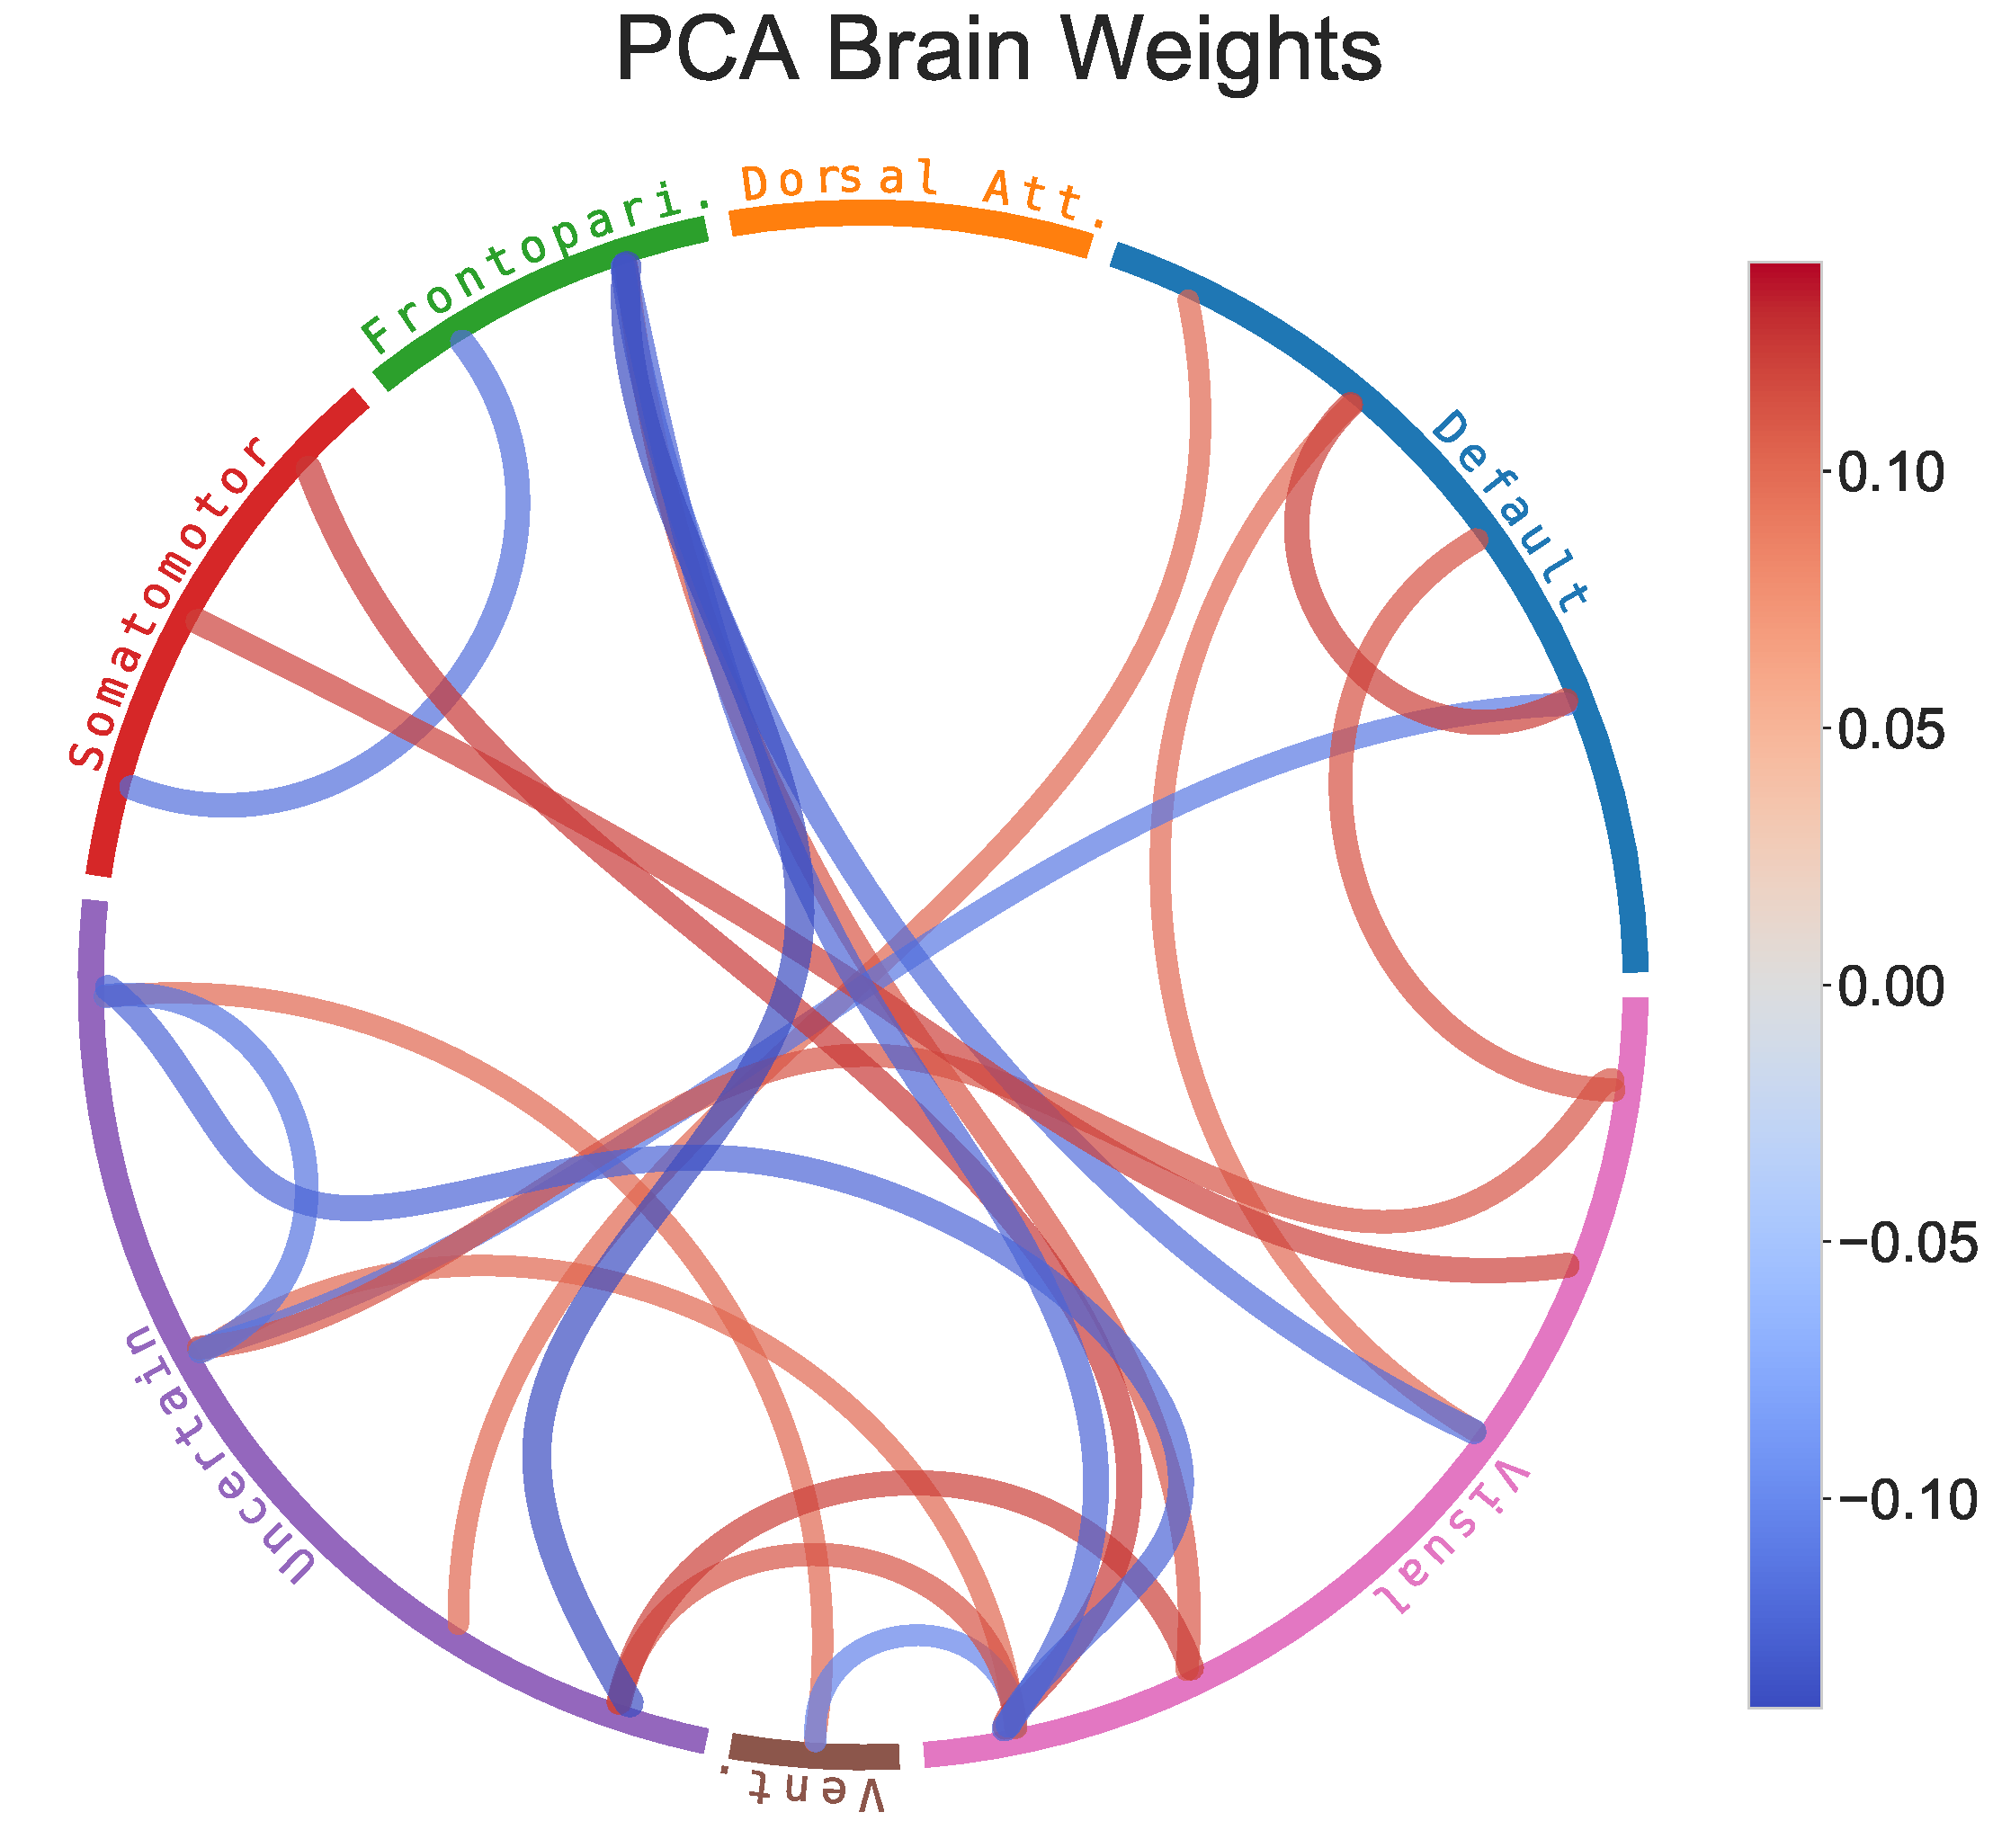
\includegraphics[width=0.49\linewidth]{figures/hcp/PCA brain weights}
    \caption{\textbf{HCP:} Chord diagrams of the top 8 positive and negative brain \gls{weights} for each model.}\label{fig:chord_weights}
\end{figure}

\subsubsection{Model Similarity}

In this section, we compare the models in terms of their similarity.
We can measure the pairwise similarity between two models by comparing their \gls{weights} and their \gls{representations}.
We can compare the \gls{weights} by computing the correlation between the \gls{weights} of the two models and we can compare the \gls{representations} by computing the correlation between the \gls{representations} of the two models.

In Figure~\ref{fig:brain-behaviour-scores-sim}, we plot the correlation between the brain and behaviour \gls{representations} for each model. 
We can see clearly that both PCA, PLS, and SPLS are all highly correlated in terms of their brain representations, revealing the bias of PLS towards the largest principal components.
On the other hand, in the behaviour space, the models are less correlated, with the exception of PLS and SPLS which are highly correlated with one another. 
There is however still substantial correlation between the PCA and PLS models.
The very low correlation between the Ridge CCA and Elastic Net models with the PCA model is evidence that there are stronger correlations outside of the first principal components.

In Figure~\ref{fig:brain-behaviour-weights-sim}, we similarly plot the correlation between the brain and behaviour \gls{weights} for each model. 
The story is similar, albeit with marginally lower correlations between the PLS and PCA-based models. Finally, in the weights space, the Ridge CCA and ElasticNet models are even less correlated with the PCA model.

\begin{figure}
    \centering
    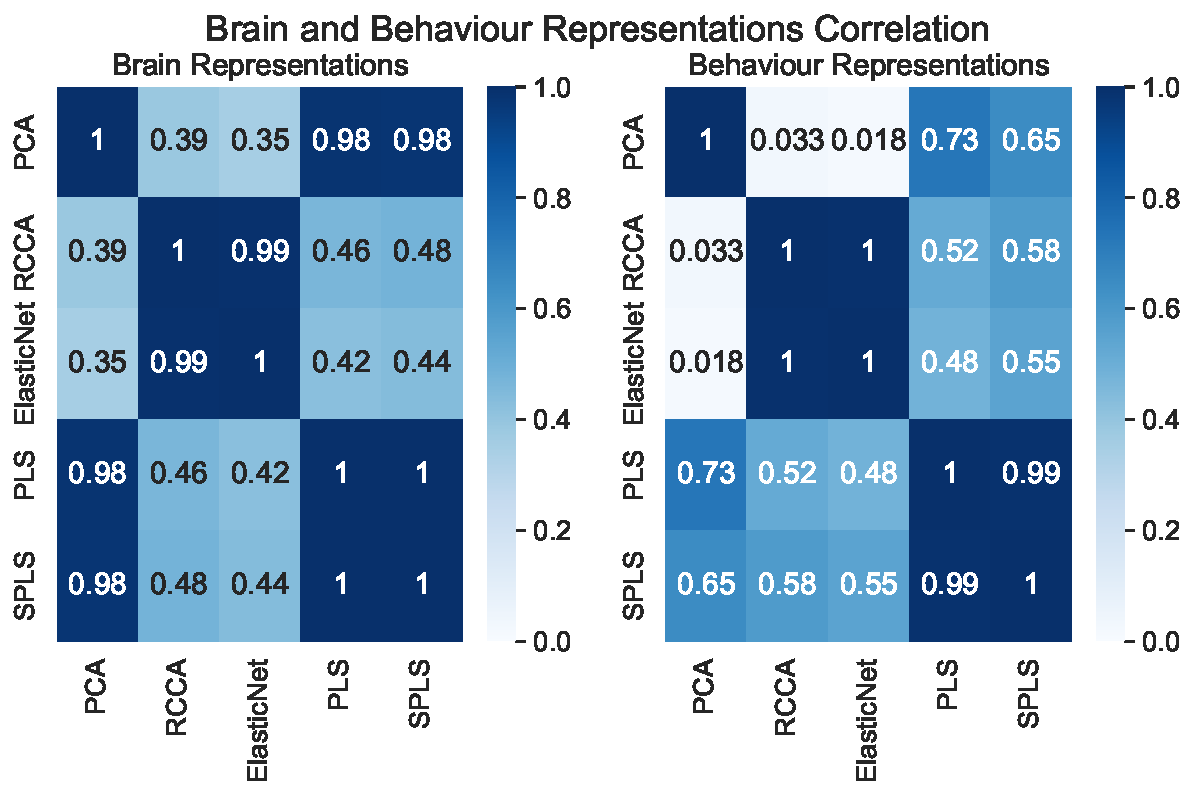
\includegraphics[width=0.8\linewidth]{figures/hcp/brain and behaviour scores correlation}
    \caption{\textbf{HCP:} Correlation between the brain and behaviour \gls{representations} for each model.}\label{fig:brain-behaviour-scores-sim}
\end{figure}

\begin{figure}
    \centering
    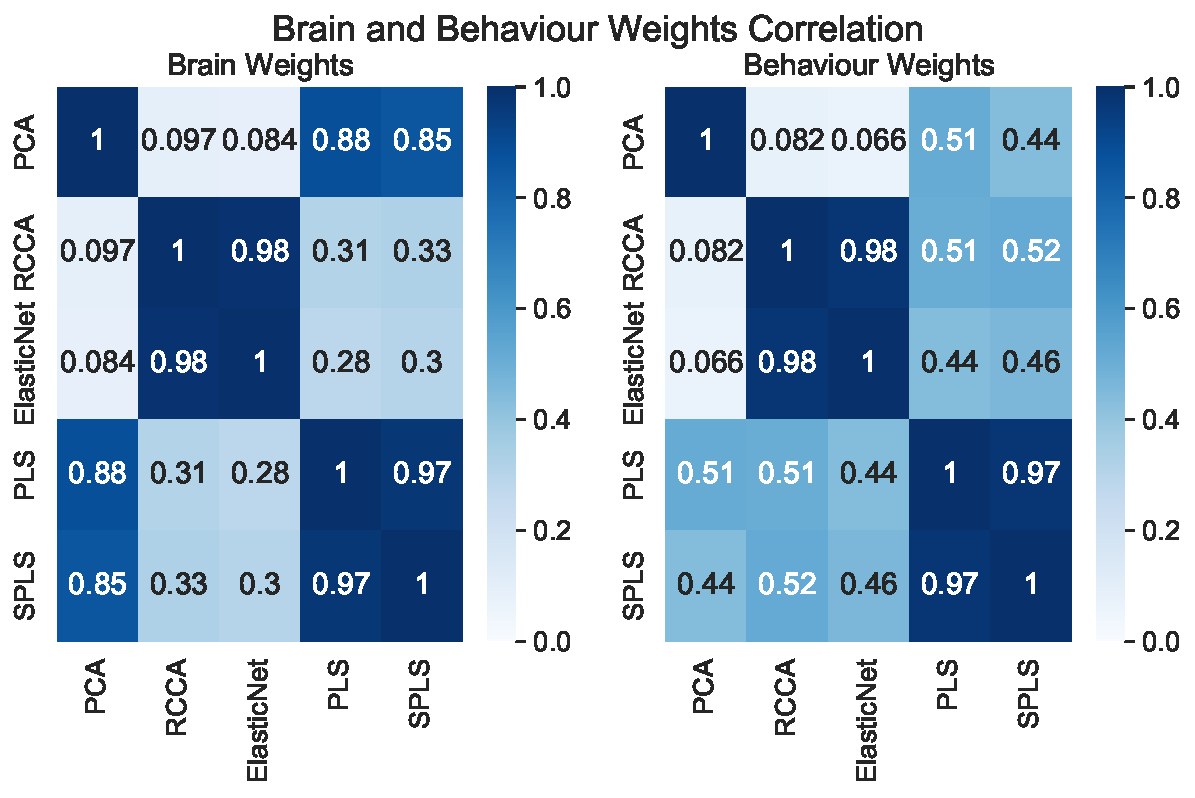
\includegraphics[width=0.8\linewidth]{figures/hcp/brain and behaviour weights correlation}
    \caption{\textbf{HCP:} Correlation between the brain and behaviour \gls{weights} for each model.}\label{fig:brain-behaviour-weights-sim}
\end{figure}


\subsection{\acrshort{adni} Results}\label{subsec:adni}

We now turn to the \acrshort{adni} data.

\subsubsection{Out of Sample Correlation}

In this experiment, the Elastic Net model outperformed all other models in terms of out-of-sample correlation (Figure~\ref{fig:performance}).
The RCCA model also outperformed the PLS and SPLS models while SPLS outperformed PLS.
Suprisingly, PCA performed almost as well as PLS.
This suggests that there is value in both tunable shrinkage and sparsity in this dataset.
It also reveals that the correlated signal between the brain structure and behavioural data is relatively much stronger than in the \acrshort{hcp} data.

\begin{figure}
    \centering
    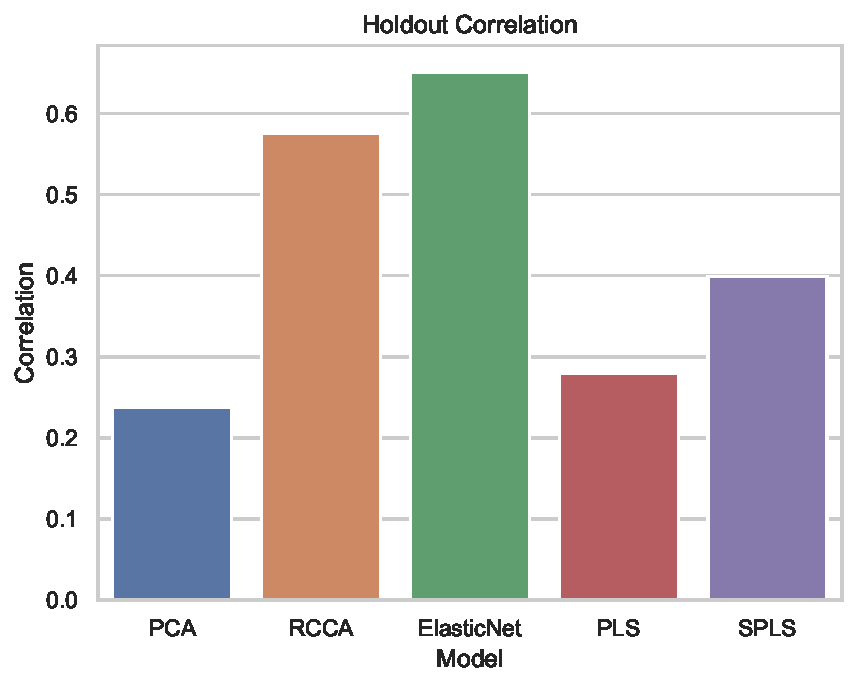
\includegraphics[width=0.5\linewidth]{figures/adni/holdout_correlations}
    \caption{\textbf{ADNI:} Out-of-sample canonical correlations for each model.}\label{fig:performance}
\end{figure}

\subsubsection{Sparsity of Weights}

Table~\ref{tab:brain-behaviour-weights-adni} once again shows the number of non-zero \gls{weights} for each model.
We can see that tuned SPLS and Elastic Net once again identify sparse weights.
In this case, the difference in performance is more convincing and suggests that this sparsity is less spuriously induced than for the \acrshort{hcp} data.
This is supported by the fact that Elastic Net and SPLS models find a similar level of sparsity in the brain weights.
On the other hand SPLS finds a much sparser set of behavioural weights.

\begin{table}
    \centering
    \caption{\textbf{ADNI:} Number of non-zero \gls{weights} for each model.}
    \begin{tabular}{|c|c|c|}
        \hline
        Model       & Brain Weights & Behaviour Weights \\
        \hline
        PCA         & 168130        & 31                \\
        RCCA        & 168130        & 31                \\
        Elastic Net & 59617         & 17                \\
        PLS         & 168130        & 31                \\
        SPLS        & 74995         & 10                \\
        \hline
    \end{tabular}\label{tab:brain-behaviour-weights-adni}
\end{table}

\subsubsection{Behaviour Weights}

As for the \acrshort{hcp} data, Figure \ref{fig:adni-beh} plots the top 8 positive and negative non-imaging \gls{weights} for each model.
Some of the identified behavioural \gls{weights} including a number of orientation tests are similar across all of the models, including even PCA.
This is indicative of the strong shared signal between the behavioural data and the brain structure data.
SPLS and Elastic Net both emphasize the orientation and recall tests in the weight space.
The RCCA and Elastic Net models are suprisingly different in the weight space, with the RCCA \gls{weights} on a couple of attention and calculation tests in addition to the ubiquitous orientation and recall tests.

\begin{figure}
    \centering
    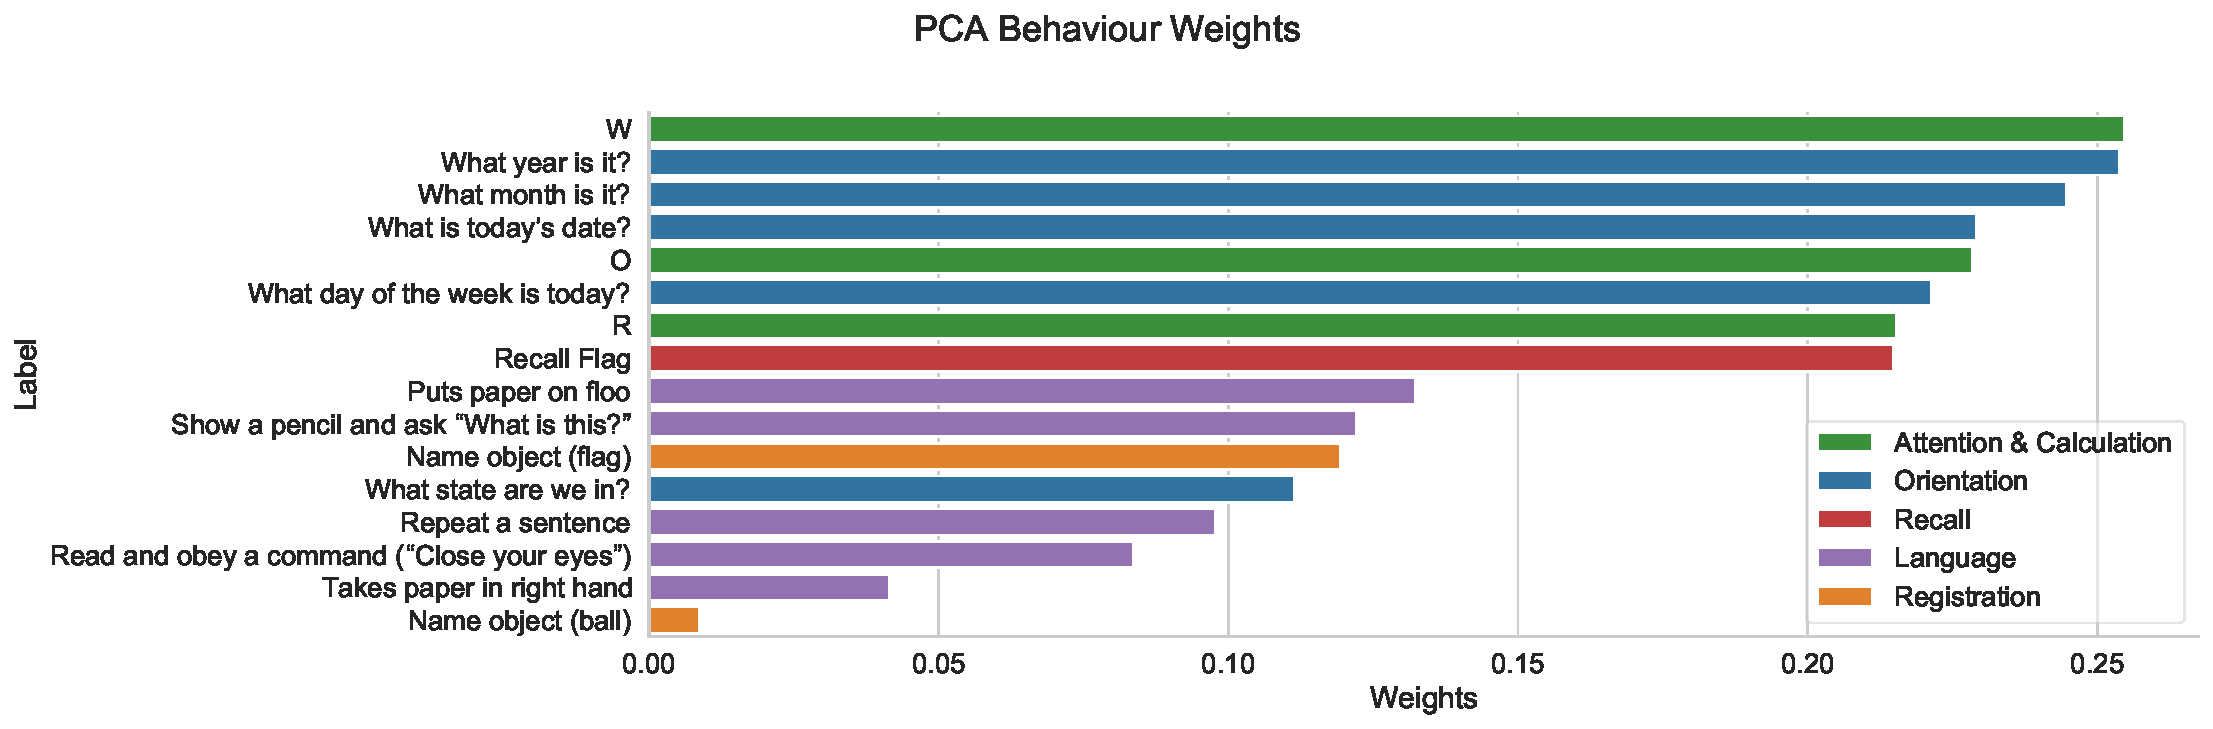
\includegraphics[width=0.8\linewidth]{figures/adni/PCA behaviour weights}
    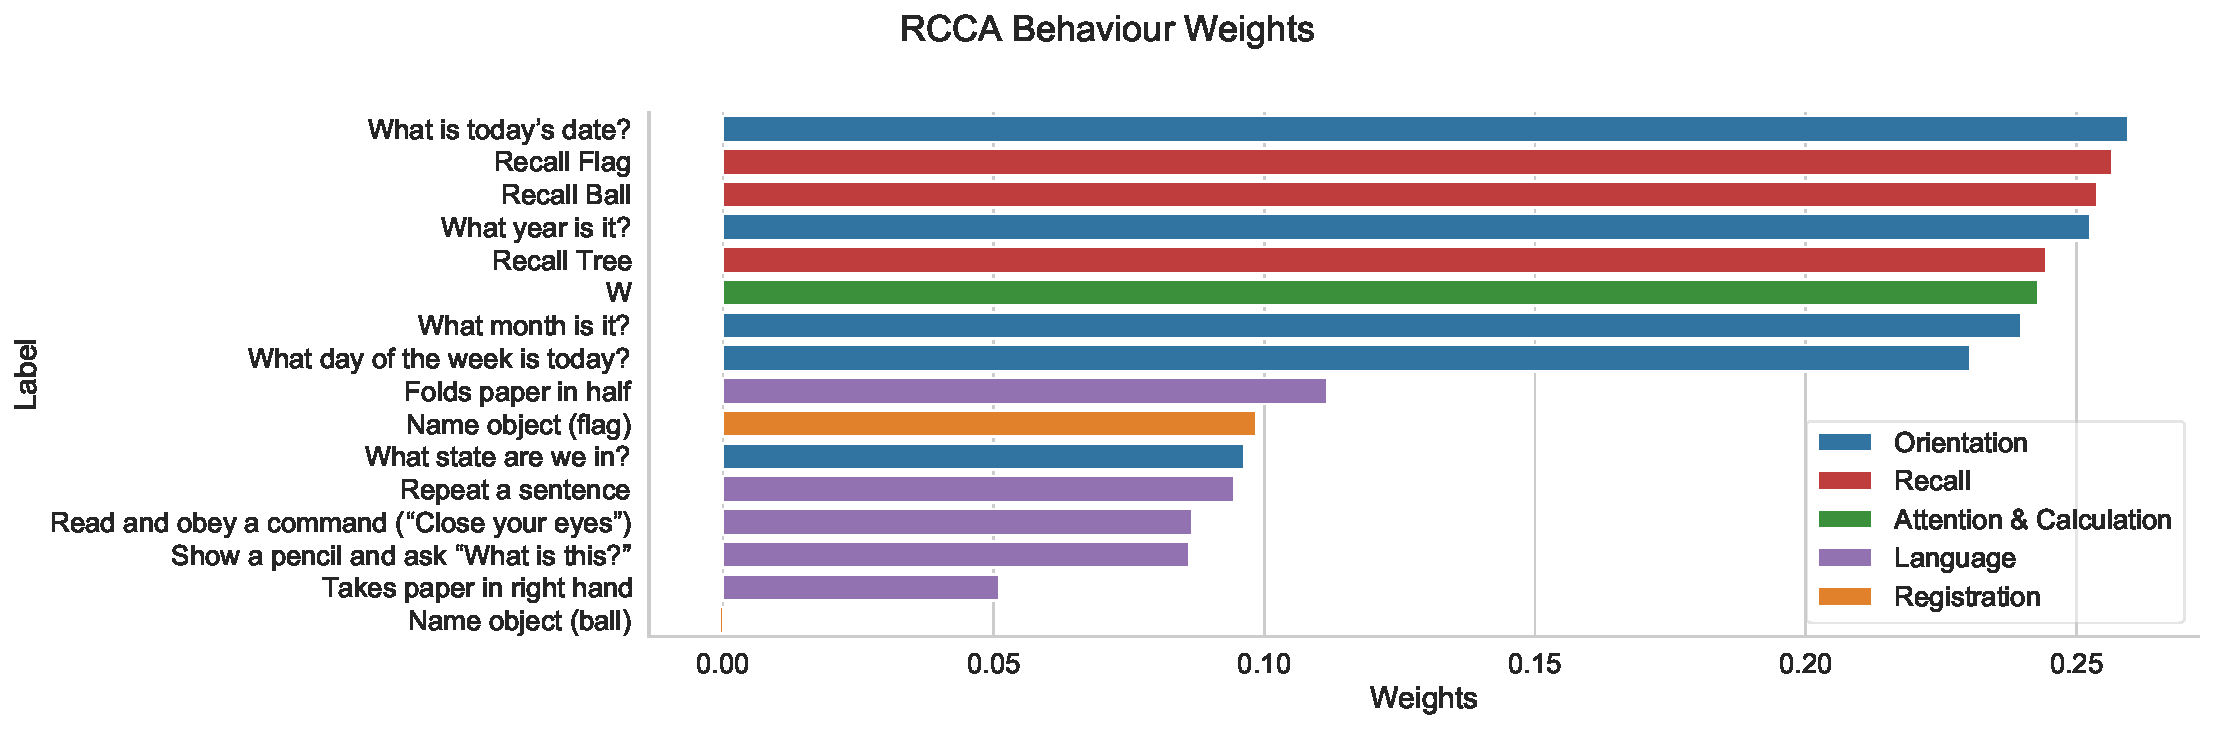
\includegraphics[width=0.8\linewidth]{figures/adni/RCCA behaviour weights}
    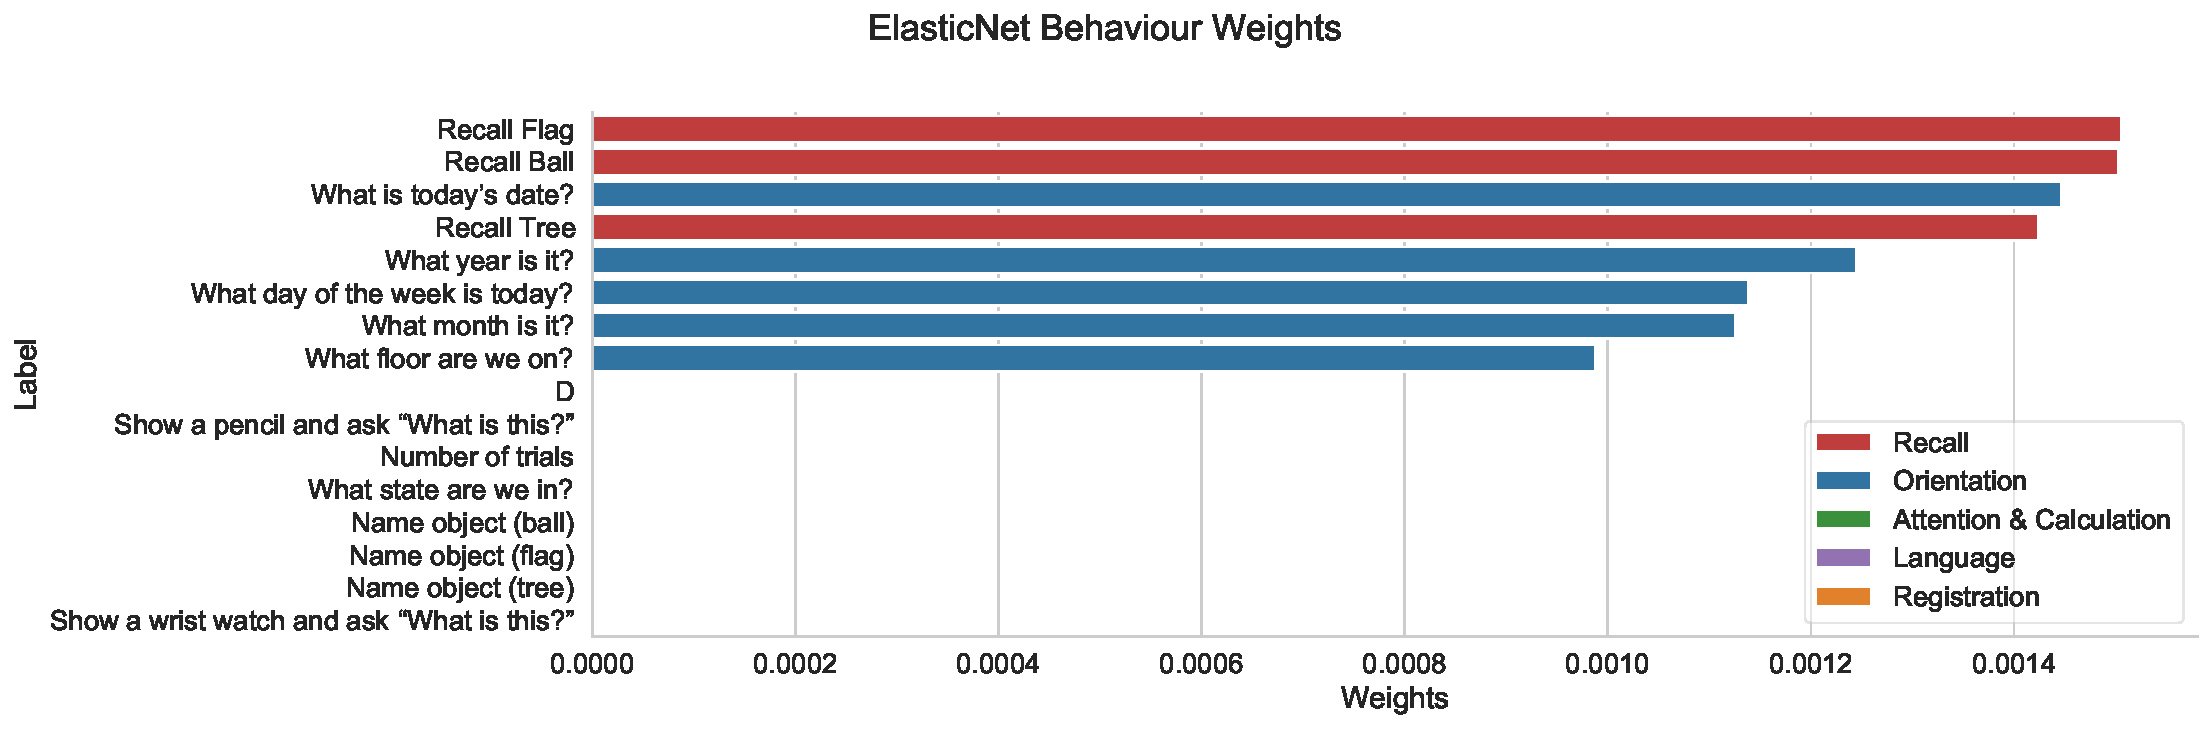
\includegraphics[width=0.8\linewidth]{figures/adni/ElasticNet behaviour weights}
    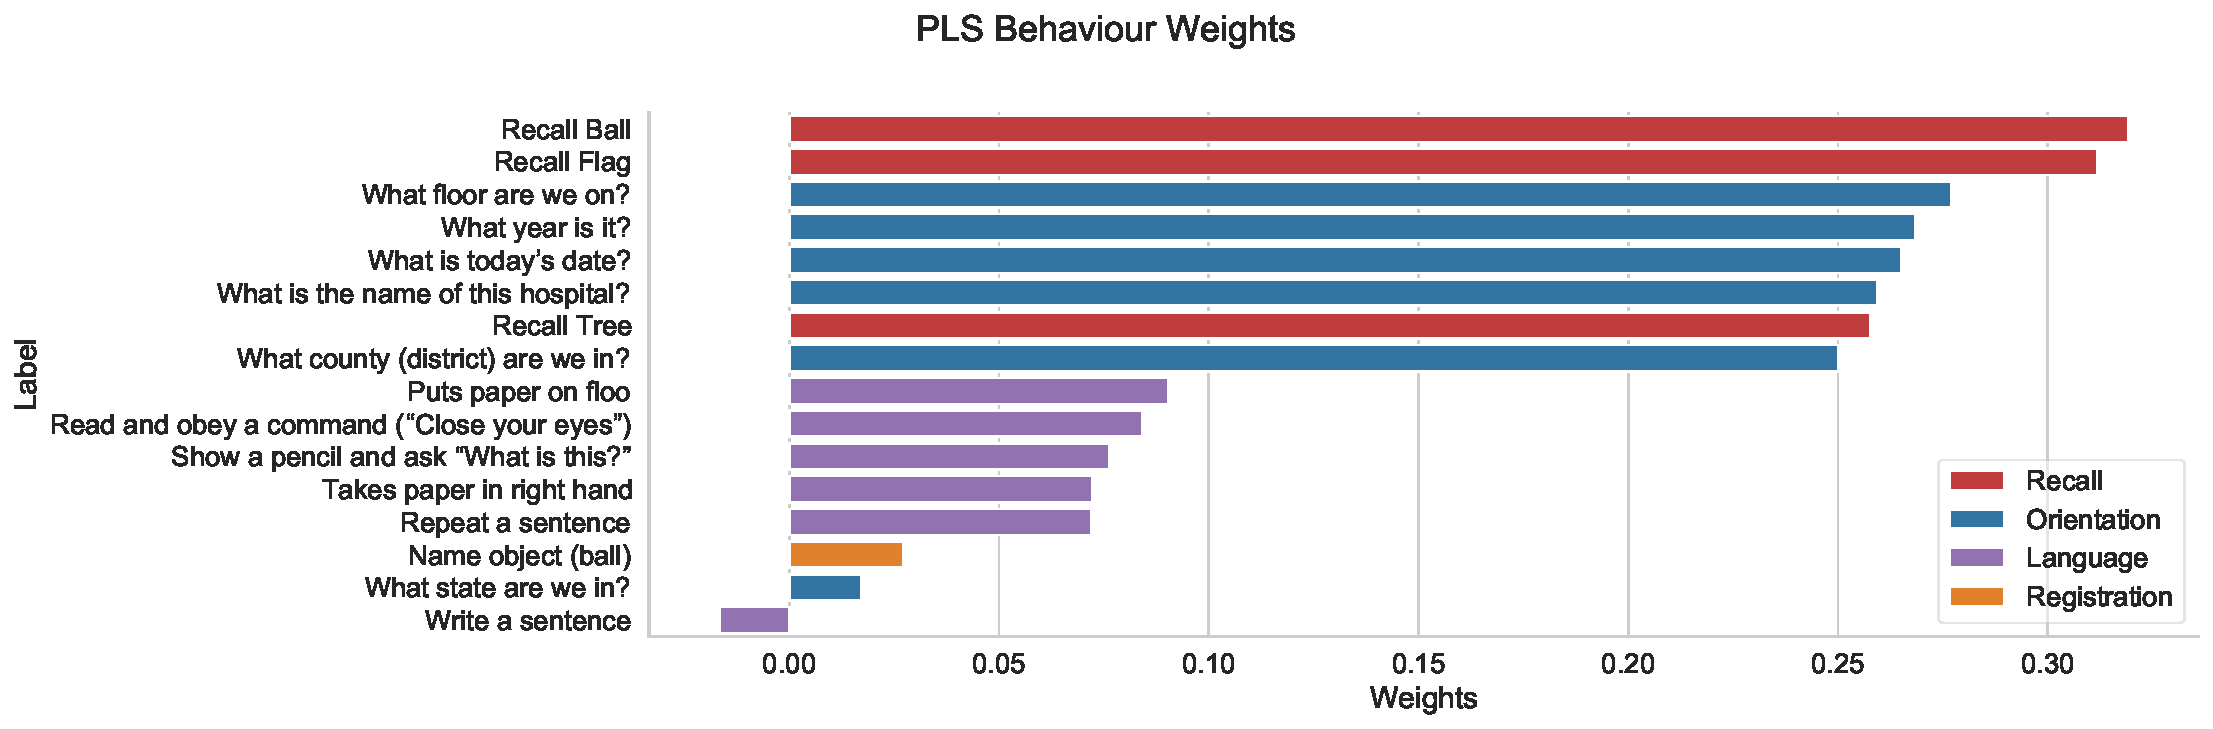
\includegraphics[width=0.8\linewidth]{figures/adni/PLS behaviour weights}
    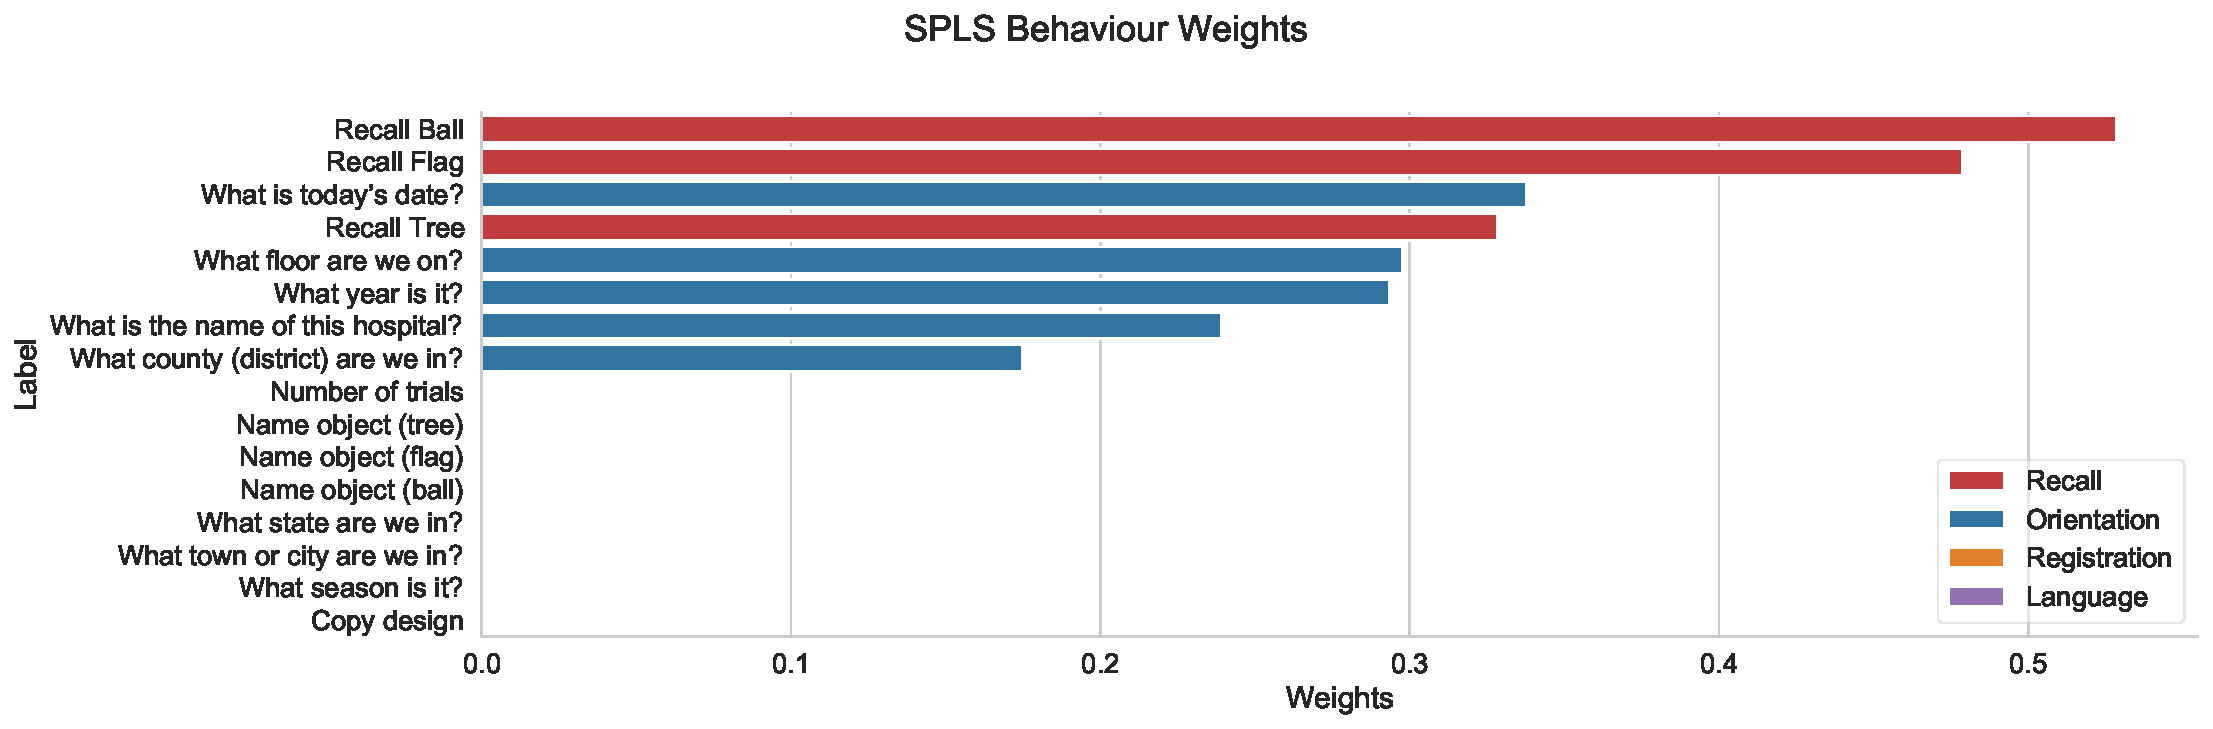
\includegraphics[width=0.8\linewidth]{figures/adni/SPLS behaviour weights}
    \caption{\textbf{ADNI:} Bar plots of the behaviour \gls{weights} for each model.}\label{fig:adni-beh}
\end{figure}

\subsubsection{Brain Structure Weights}

We plot the \gls{weights} as a mosaic plot with 3 slices in each direction in Figure~\ref{fig:adni-brain}.
Previous work using SPLS with the \acrshort{adni} dataset identified the same striking pattern of \gls{weights} with the model strikingly selecting the hippocampal weights \citep{monteiro2016multiple}.
The Elastic Net has a less visually appealing selection of weights, with a honeycomb pattern near the edges of the brain and likewise for RCCA.
It is noticeable that PCA, PLS and SPLS both \gls{weights} in the same direction whereas RCCA and Elastic Net weight different regions with opposite signs.

\begin{figure}
    \centering
    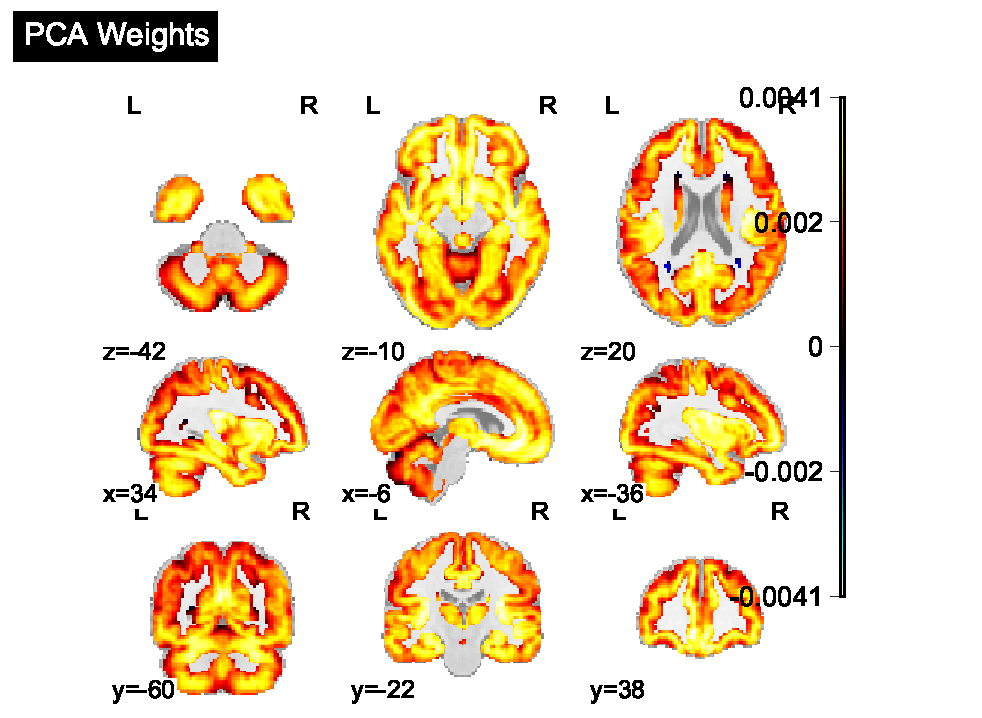
\includegraphics[width=0.45\linewidth]{figures/adni/PCA brain weights mosaic}
    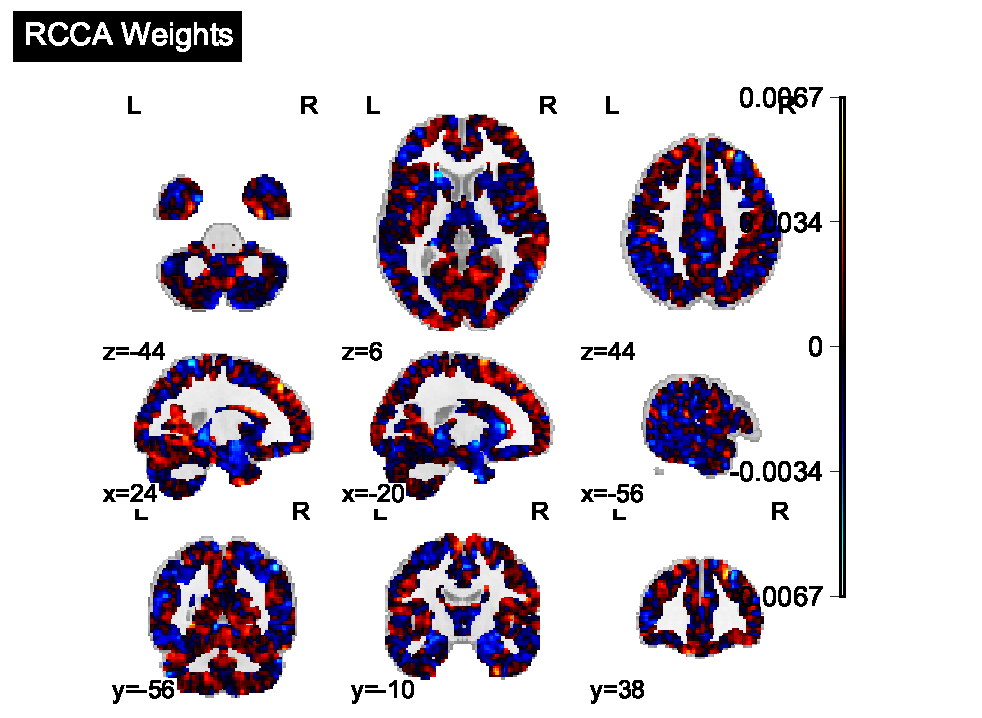
\includegraphics[width=0.45\linewidth]{figures/adni/RCCA brain weights mosaic}
    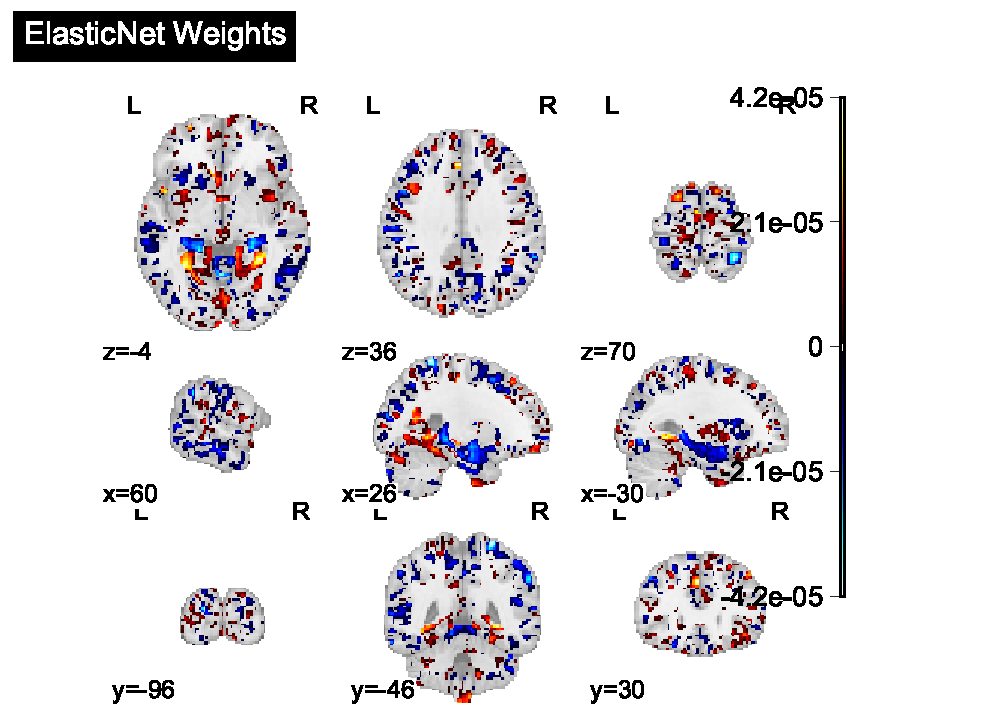
\includegraphics[width=0.45\linewidth]{figures/adni/ElasticNet brain weights mosaic}
    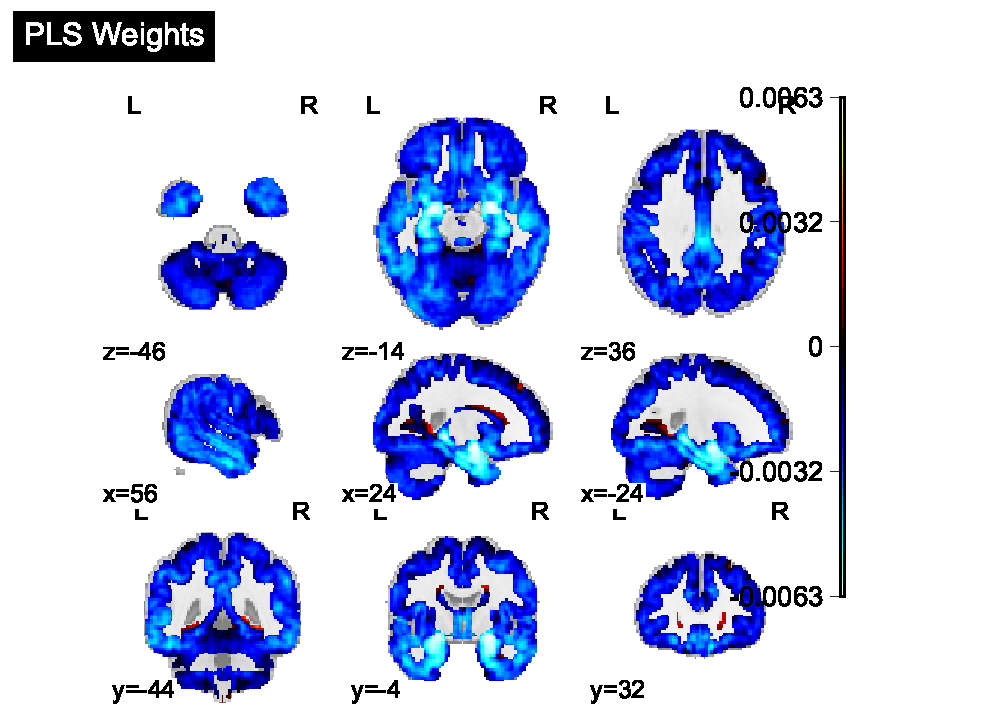
\includegraphics[width=0.45\linewidth]{figures/adni/PLS brain weights mosaic}
    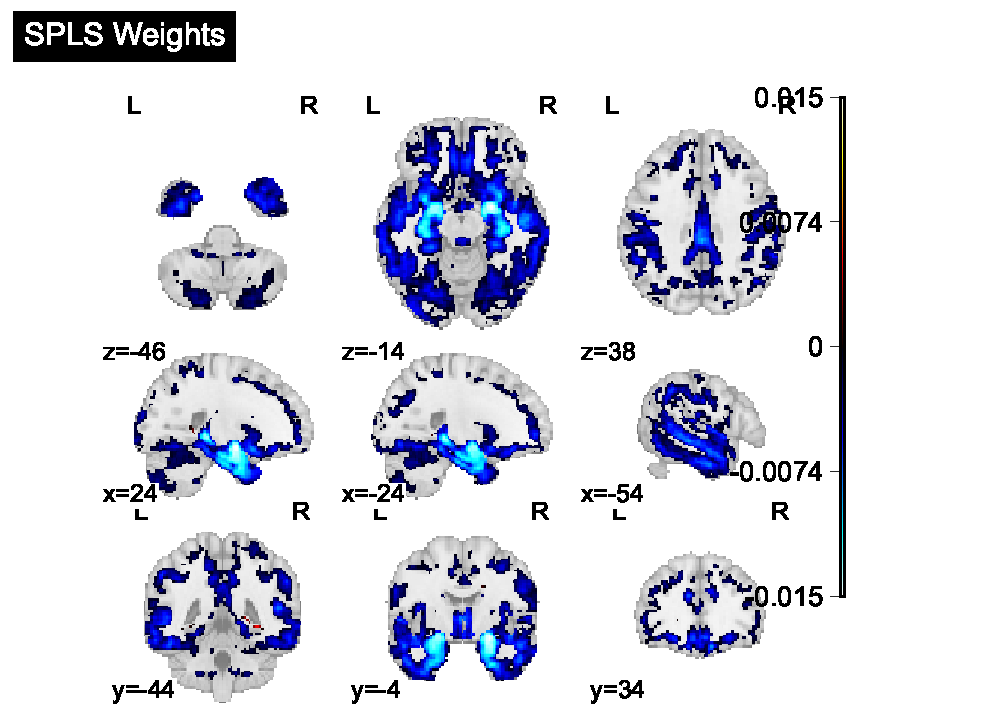
\includegraphics[width=0.45\linewidth]{figures/adni/SPLS brain weights mosaic}
    \caption{\textbf{ADNI:} Statistical maps of brain structure weights for each model.}
\end{figure}

\subsubsection{Model Similarity}

In this section, we once again compare the models in terms of their similarity.
In Figure~\ref{fig:brain-behaviour-scores-sim-adni}, we can see that all of the models are highly correlated in terms of their behaviour \gls{representations}.
The brain \gls{representations} are less correlated, but once again PCA, PLS, and SPLS are highly correlated with one another and less correlated with the Ridge CCA and Elastic Net models.

Suprisingly, in Figure~\ref{fig:brain-behaviour-weights-sim-adni}, we can see that the weights in both views are less correlated. This is particularly true for the brain \gls{weights} where PCA exhibits a very low correlation with Ridge CCA and Elastic Net.

\begin{figure}
    \centering
    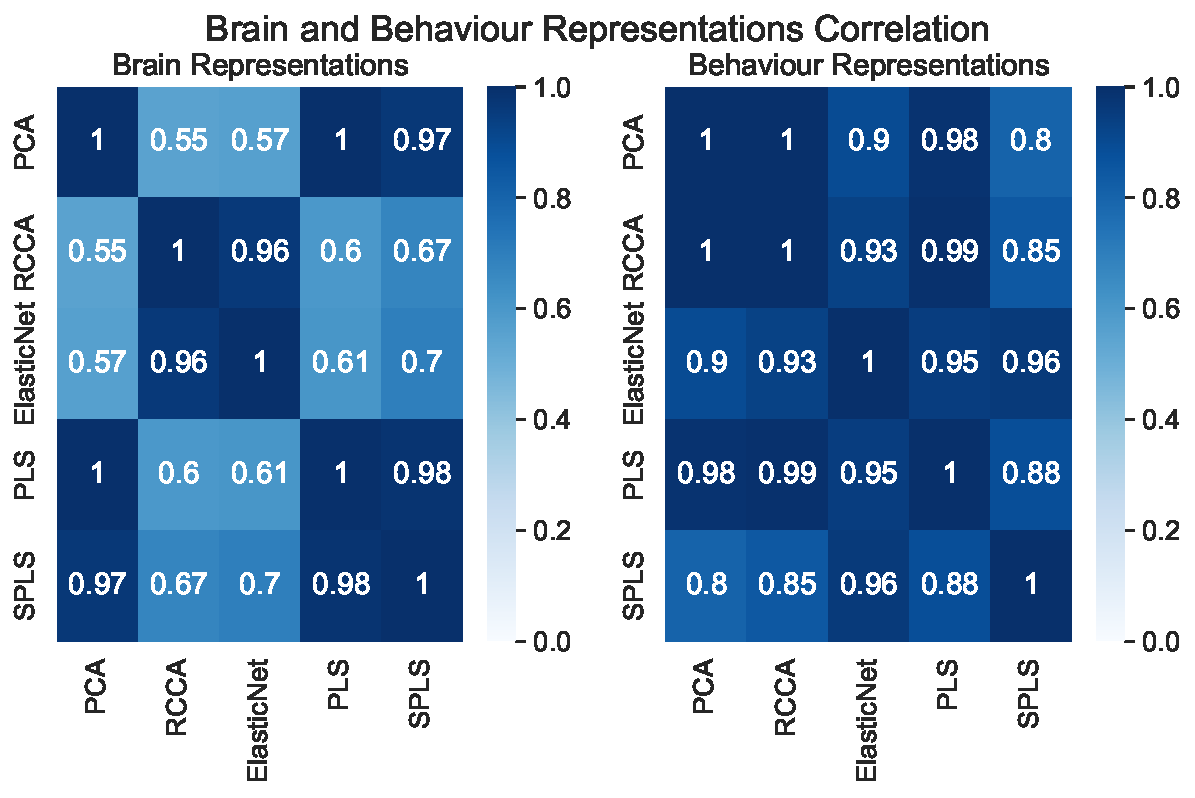
\includegraphics[width=0.8\linewidth]{figures/adni/brain and behaviour scores correlation}
    \caption{\textbf{ADNI:} Correlation between the brain and behaviour \gls{representations} for each model.}\label{fig:brain-behaviour-scores-sim-adni}
\end{figure}

\begin{figure}
    \centering
    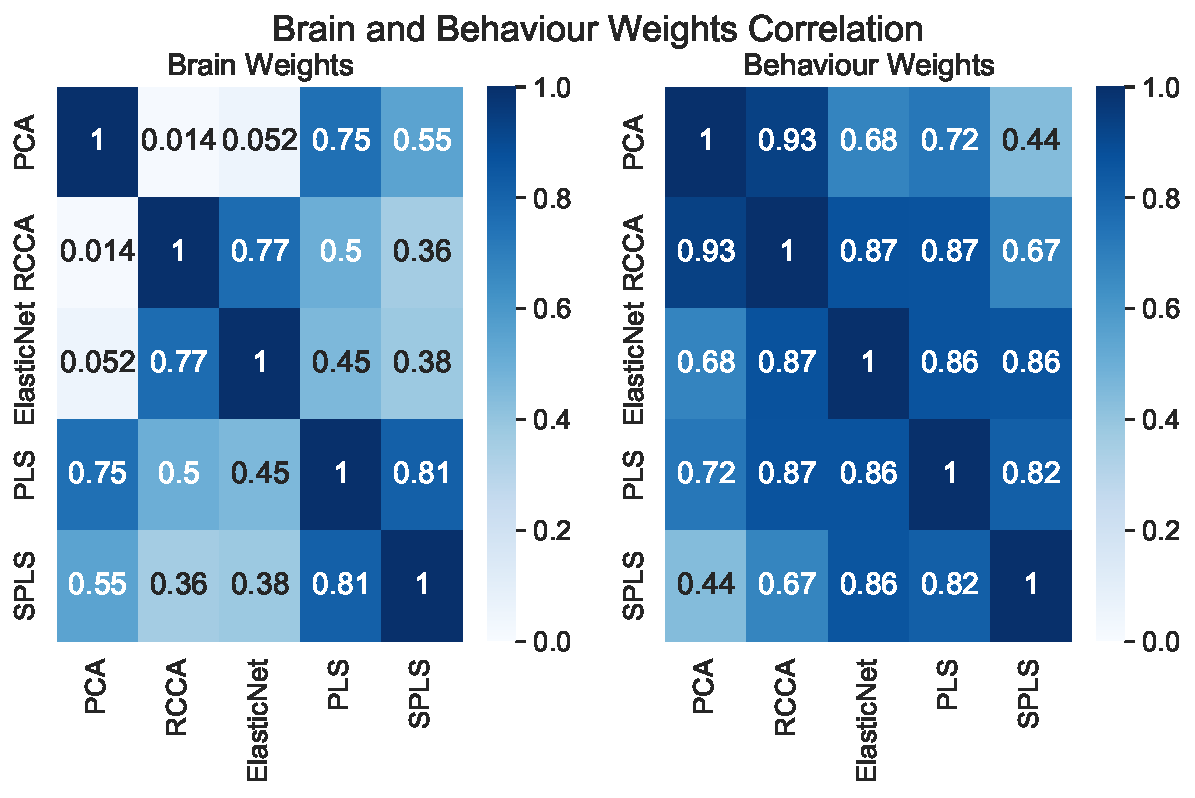
\includegraphics[width=0.8\linewidth]{figures/adni/brain and behaviour weights correlation}
    \caption{\textbf{ADNI:} Correlation between the brain and behaviour \gls{weights} for each model.}\label{fig:brain-behaviour-weights-sim-adni}
\end{figure}

\subsection{Timings}

Finally, we consider the timings of the different models.
This is an important metric because one of the main reasons for the popularity of SPLS is its speed and therefore convenience.
Figure \ref{fig:timings} shows an estimate of the time taken to fit each model for each complete training dataset over 10 runs.
We can see clearly that the Elastic Net is much slower than the other models when using the high dimensional \acrshort{adni} data.
Despite also being an iterative algorithm, the SPLS model is much faster than the Elastic Net and only slightly slower than the PLS and RCCA models which call optimised solvers in C.
Since PLS and RCCA both use PCA preprocessing for efficiency, it is unsuprising that PCA is the fastest model.

\begin{figure}
    \centering
    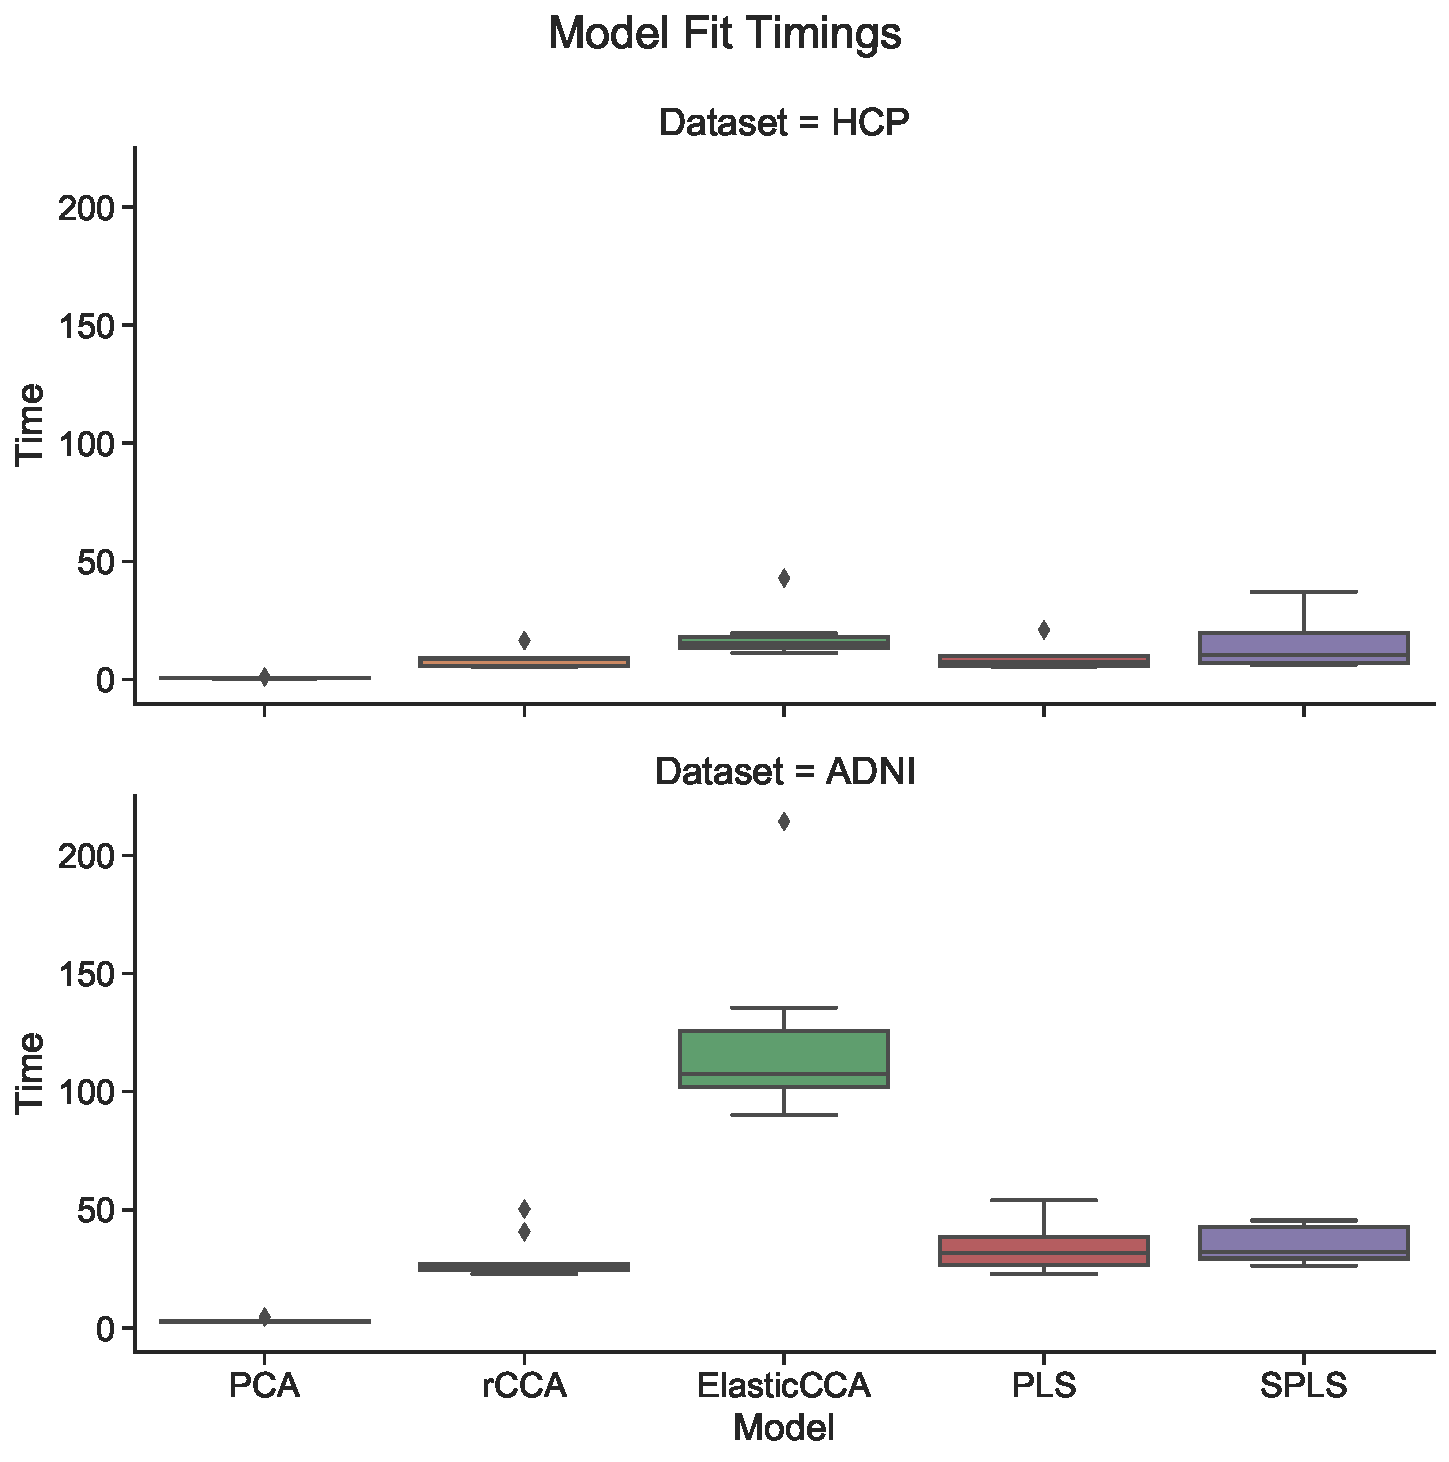
\includegraphics[width=0.45\linewidth]{figures/model_fit_timings}
    \caption{Time taken to fit each model.}\label{fig:timings}
\end{figure}

\section{Discussion and Limitations}

In this section, we discuss the implications of our findings as well as the limitations of our study and the proposed FRALS method, some of which we address in later chapters of this thesis.

\subsection{Discussion}

\paragraph{Ridge CCA is typically much better than PLS across datasets:} Our results show that Ridge CCA is typically much better than PLS across datasets.
Much like regularised regression, it is unusual to need to use maximal ridge regularisation even in high dimensions.
This means that while PLS might be more stable for a given dataset, it is not necessarily more stable across random samples from the same population.

\subsection{FRALS Limitations}
While FRALS offers promising performance in terms of out-of-sample correlation, it does come with significant drawbacks, the most noteworthy being its computational inefficiency.
Below, we outline the primary factors contributing to the slow speed of FRALS and provide some insights into the computational bottlenecks.

\paragraph{Changing Regression Targets}\label{subsec:changing-regression-targets}
Adding to the computational burden is the fact that the regression targets, i.e., the projections of the other view, are not static but change dynamically throughout the algorithm's run.
Each update to the least squares solution consequently alters the global objective, leading to a constantly shifting landscape that the algorithm needs to navigate.
This also leads to a significant amount of redundant computation, as the algorithm needs to recompute the least squares solution for each view at each iteration.

\paragraph{Computational Time}\label{subsec:computational-time}

The primary bottleneck in FRALS is the computation of the least squares solution.
For each iteration of the algorithm, we need to compute the least squares solution for each view.
This is a computationally expensive operation.
It is the primary factor contributing to the slow speed of FRALS (depending on the experiment around 10 times slower than Ridge CCA).

\section{Conclusion}\label{sec:conclusion}

In this chapter, we introduced the Flexible Regularised Alternating Least Squares (FRALS) framework for CCA\@.
We used the FRALS framework to implement Elastic Net CCA\@.
We then compared the performance of Elastic Net CCA with other CCA variants on two datasets: the \acrshort{hcp} and \acrshort{adni}.
We found that Elastic Net CCA outperformed other CCA variants on both datasets but that the performance of Elastic Net CCA was similar to Ridge CCA on the \acrshort{hcp} dataset.
However, we found that Elastic Net CCA was much slower than other CCA variants.
